\chapter{Gravitational radiation in $f(R)$-gravity\label{ch:f-R1}}

\section{Beyond general relativity: $f(R)$ modified gravity}

GR is a well tested theory of gravity \citep{Will2006}. However, there are many unanswered questions that remain regarding gravity which motivate the exploration of alternate theories: What are the true natures of dark matter and dark energy? How should we formulate a quantizable theory of gravity? What drove inflation in the early Universe?  Is GR the only theory that is consistent with current observations? Moreover, the majority of the tests that have been carried out to date have been in the weak-field, low-energy regime \citep{Will2006, Will1993,Psaltis2008a}. It is not unreasonable to suspect there may be higher order corrections that are only discovered in the strong-field regime, where curvature is high or spacetime dynamic.

In this and the following chapter, we shall study a modified theory of gravitation to assess the feasibility of potential corrections to GR. We investigate metric $f(R)$-gravity, in which the Einstein-Hilbert action is modified by replacing the Ricci scalar $R$ with an arbitrary function $f(R)$. This is one of the simplest extensions to standard GR \citep{Sotiriou2010, DeFelice2010}. It has attracted significant interest because the flexibility in defining the function $f(R)$ allows a wide range of cosmological phenomena to be described \citep{Nojiri2007, Capozziello2007a}. For example, \citet{Starobinsky1980} suggested that a quadratic addition to the field equations could drive exponential expansion of the early Universe \citep{Vilenkin1985}: inflation in modern terminology. In this model $f(R) = R - R^2/(6\Upsilon^2)$; the size of the quadratic correction can be tightly constrained by considering the spectrum of curvature perturbations generated during inflation \citep{Starobinskii1983, Starobinskii1985}. Using the results of the Wilkinson Microwave Anisotropy Probe (WMAP; \citealt{Bennett2012, Hinshaw2012}), the inverse length-scale can be constrained to $\Upsilon \simeq 3 \times 10^{-6} (50/N) \ell\sub{P}^{-1}$, where $N$ is the number of e-folds during inflation and $\ell\sub{P}$ is the Planck length \citep{Starobinsky2007, DeFelice2010}.

We consider simple $f(R)$ corrections within the framework of linearized gravity and discover how GWs are modified. We begin by reviewing the properties of the $f(R)$ field equations. From these, we derive the linearized equations (\secref{Lin}) and use these to determine the properties of GWs (\secref{Rad}). These are largely known in the literature, but are worked out here {\it ab initio}. We proceed to derive an effective energy-momentum tensor for gravitational radiation in \secref{EM_tensor}, following the short-wavelength approximation of \citet{Isaacson1968, Isaacson1968a}.

Following on from the theory developed in this chapter, in \chapref{f-R2} we consider observational tests of $f(R)$-gravity. We explore what constraints LISA, Solar System tests and laboratory experiments can place on the form of $f(R)$. We do not consider cosmological implications where terms beyond linear order could play a significant role. The overall conclusion is that LISA could place constraints on $f(R)$-gravity which may be more powerful than those in the Solar System, but are not as powerful as constraints from laboratory experiments. A brief summary of findings from both chapters is found in \secref{f_Discuss}.

Natural units with $c = 1$ are used throughout both chapters, but factors of $G$ are retained.

\section{Description of $f(R)$-gravity}

\subsection{The action and field equations\label{sec:Action}}

General relativity can be derived from the Einstein-Hilbert action (\citealt[chapter 21]{Misner1973}; \citealt[section 93]{Landau1975}; \citealt[section 26]{Dirac1996})
\begin{equation}
S\sub{EH}[g] = \recip{16\pi G}\intd{}{}{R\sqrt{-g}}{^4x}.
\end{equation}
In $f(R)$ theory we make a simple modification of the action to include an arbitrary function of the Ricci scalar $R$ such that \citep{Buchdahl1970}
\begin{equation}
S_{f(R)}[g] = \recip{16\pi G}\intd{}{}{f(R)\sqrt{-g}}{^4x}.
\end{equation}
Including the function $f(R)$ gives extra freedom in defining the behaviour of gravity. While this action may not encode the true theory of gravity it could contain sufficient information to act as an effective field theory, correctly describing phenomenological behaviour \citep{Park2010}; it may be that as an effective field theory, a particular $f(R)$ shall have a limited region of applicability and shall not be universal. We assume that $f(R)$ is analytic about $R = 0$ so that it can be expressed as a power series \citep{Buchdahl1970, Capozziello2007, Faulkner2007, Clifton2008, Psaltis2008}
\begin{equation}
f(R) = a_0 + a_1 R + \frac{a_2}{2!}R^2 + \frac{a_3}{3!}R^3 + \ldots
\end{equation}
Since the dimensions of $f(R)$ must be the same as of $R$, $[a_n] = [R]^{(1-n)}$. To link to GR we set $a_1 = 1$; any rescaling can be absorbed into the definition of $G$.

Various models of cosmological interest may be expressed in such a form, for example, the model of \citet{Starobinsky2007}
\begin{equation}
f(R) = R + \lambda R_0 \left[\left(1 + \frac{R^2}{R_0^2}\right)^{-n} - 1\right],
\end{equation}
can be expanded as
\begin{equation}
f(R) = R - \frac{\lambda n}{R_0} R^2 + \frac{\lambda n (n + 1)}{2 R_0^3} R^4 + \ldots
\end{equation}
Consequently such a series expansion can constrain model parameters, although we cannot specify the full functional form from only a few terms.

The field equations are obtained by a variational principle; there are several ways of achieving this. To derive the Einstein field equations from the Einstein-Hilbert action one may use the standard metric variation or the Palatini variation \citep[section 21.2]{Misner1973}. Both approaches can be used for $f(R)$, but they yield different results \citep{Sotiriou2010, DeFelice2010}. Following the metric formalism, one varies the action with respect to the metric $g^{\mu\nu}$. Following the Palatini formalism one varies the action with respect to both the metric $g^{\mu\nu}$ and the connection ${\Gamma^\rho}_{\mu\nu}$, which are treated as independent quantities: the connection is not the Levi-Civita metric connection.\footnote{Imposing the condition that the metric and Palatini formalisms produce the same field equations, assuming an action that only depends on the metric and Riemann tensor, results in Lovelock gravity \citep{Exirifard2008}. Lovelock gravities require the field equations to be divergence free and no more than second order; in four dimensions the only possible Lovelock gravity is GR with a potentially non-zero cosmological constant \citep{Lovelock1970, Lovelock1971, Lovelock1972}.}

Finally, there is a third version of $f(R)$-gravity: metric-affine $f(R)$-gravity \citep{Sotiriou2007, Sotiriou2007b}. This goes beyond the Palatini formalism by supposing that the matter action is dependent on the variational independent connection. Parallel transport and the covariant derivative are divorced from the metric. This theory has its attractions: it allows for a natural introduction of torsion. However, it is not a metric theory of gravity and so cannot satisfy all the postulates of the Einstein equivalence principle \citep{Will2006}: a free particle does not necessarily follow a geodesic and so the effects of gravity might not be locally removed \citep{Exirifard2008}. The implications of this have not been fully explored, but for this reason we will not consider the theory further.

We restrict our attention to metric $f(R)$-gravity. This is preferred as the Palatini formalism has undesirable properties: static spherically symmetric objects described by a polytropic equation of state are subject to a curvature singularity \citep{Barausse2008b, Barausse2008a, DeFelice2010}. Varying the action with respect to the metric $g^{\mu\nu}$ produces
\begin{align}
\delta S_{f(R)} = {} & \recip{16\pi G}\int\left\{f'(R)\sqrt{-g}\left[R_{\mu\nu} - \nabla_\mu\nabla_\nu\ + g_{\mu\nu}\Box\right] \hphantom{\frac{0}{0}} \vphantom{\frac{0}{0}} - f(R)\recip{2}\sqrt{-g}g_{\mu\nu}\right\}\delta g^{\mu\nu}\,\dd^4x,
\end{align}
where $\Box = g^{\mu\nu}\nabla_\mu\nabla_\nu$ is the d'Alembertian and a prime denotes differentiation with respect to $R$.

Proceeding from here requires certain assumptions regarding surface terms. In the case of the Einstein-Hilbert action these gather into a total derivative; it is possible to subtract this from the action to obtain a well-defined variational quantity \citep{York1972, Gibbons1977}. This is not the case for general $f(R)$-gravity \citep{Madsen1989}. However, since the action includes higher-order derivatives of the metric, we are at liberty to fix more degrees of freedom at the boundary, in so doing eliminating the importance of the surface terms \citep{Dyer2009a, Sotiriou2010}. Setting the variation $\delta R = 0$ on the boundary allows us to subtract a term similar to that in GR \citep{Guarnizo2010}. We then have a well-defined variational quantity, from which we can obtain the field equations.

The vacuum field equations are
\begin{equation}
f'R_{\mu\nu} - \nabla_\mu\nabla_\nu f' + g_{\mu\nu}\Box f' - \frac{f}{2}g_{\mu\nu} = 0.
\label{eq:Field_eq}
\end{equation}
Taking the trace gives
\begin{equation}
f'R + 3\Box f' - 2f = 0.
\label{eq:Trace_eq}
\end{equation}
If we consider a uniform flat spacetime $R = 0$, this requires \citep{Capozziello2007}
\begin{equation}
a_0 = 0.
\label{eq:a_0}
\end{equation}
In analogy to the Einstein tensor, we define
\begin{equation}
\mathcal{G}_{\mu\nu} = f'R_{\mu\nu} - \nabla_\mu\nabla_\nu f' + g_{\mu\nu}\Box f' - \frac{f}{2}g_{\mu\nu},
\label{eq:G_tensor}
\end{equation}
so that in a vacuum
\begin{equation}
\mathcal{G}_{\mu\nu} = 0.
\end{equation}

\subsection{Conservation of energy-momentum}

If we introduce matter with a stress-energy tensor $T_{\mu\nu}$, the field equations become
\begin{equation}
\mathcal{G}_{\mu\nu} = 8\pi GT_{\mu\nu}.
\end{equation}
Acting upon this with the covariant derivative
\begin{align}
8\pi G\nabla^\mu T_{\mu\nu} = {} & \nabla^\mu\mathcal{G}_{\mu\nu} \nonumber \\*
 = {} & R_{\mu\nu}\nabla^\mu f' + f'\nabla^\mu\left(R_{\mu\nu} - \recip{2}R g_{\mu\nu}\right) - \left(\Box\nabla_\nu - \nabla_\nu\Box\right)f'.
\end{align}
The second term contains the covariant derivative of the Einstein tensor and so is zero. The final term can be shown to be
\begin{equation}
\left(\Box\nabla_\nu - \nabla_\nu\Box\right)f' = R_{\mu\nu}\nabla^\mu f',
\end{equation}
which is a useful geometric identity \citep{Koivisto2006a}. Using this
\begin{equation}
8\pi G\nabla^\mu T_{\mu\nu} = 0.
\end{equation}
Consequently energy-momentum is a conserved quantity in the same way as in GR, as is expected from the symmetries of the action.

\section{Linearised theory\label{sec:Lin}}

We start our investigation of $f(R)$ by looking at linearised theory. This is a weak-field approximation that assumes only small deviations from a flat background, greatly simplifying the field equations. Just as in GR, the linearised framework provides a natural way to study GWs. We shall see that the linearised field equations reduce down to flat-space wave equations: GWs are as much a part of $f(R)$-gravity as of GR.

Consider a perturbation of the metric from flat Minkowski space such that
\begin{equation}
g_{\mu\nu} = \eta_{\mu\nu} + h_{\mu\nu};
\end{equation}
where, more formally, $h_{\mu\nu} = \varepsilon H_{\mu\nu}$ for a small parameter $\varepsilon$.\footnote{It is because we wish to perturb about flat spacetime that we have required $f(R)$ to be analytic about $R = 0$.} We only consider terms to $\order{\varepsilon}$. The inverse metric is then
\begin{equation}
g^{\mu\nu} = \eta^{\mu\nu} - h^{\mu\nu},
\end{equation}
where we have used the Minkowski metric to raise the indices on the right, defining
\begin{equation}
h^{\mu\nu} = \eta^{\mu\sigma}\eta^{\nu\rho}h_{\sigma\rho}.
\end{equation}
Similarly, the trace $h$ is given by
\begin{equation}
h = \eta^{\mu\nu}h_{\mu\nu}.
\end{equation}
All quantities denoted by ``$h$'' are strictly $\order{\varepsilon}$.

The linearised connection is
\begin{equation}
{{\Gamma^{(1)}}^\rho}_{\mu\nu} = \frac{1}{2}\eta^{\rho\lambda}(\partial_\mu h_{\lambda\nu} + \partial_\nu h_{\lambda\mu} - \partial_\lambda h_{\mu\nu}).
\label{eq:Lin_Gamma}
\end{equation}
To $\order{\varepsilon}$ the covariant derivative of any perturbed quantity is the same as the partial derivative. The Riemann tensor is
\begin{equation}
{{R^{(1)}}^\lambda}_{\mu\nu\rho} = \frac{1}{2}(\partial_\mu\partial_\nu h^\lambda_\rho + \partial^\lambda\partial_\rho h_{\mu\nu} - \partial_\mu\partial_\rho h^\lambda_\nu - \partial^\lambda\partial_\nu h_{\mu\rho}),
\label{eq:Lin_Riemann}
\end{equation}
where we have raised the index on the differential operator with the background Minkowski metric. Contracting gives the Ricci tensor
\begin{equation}
{R^{(1)}}_{\mu\nu} = \frac{1}{2}(\partial_\mu\partial_\rho h^\rho_\nu + \partial_\nu\partial_\rho h^\rho_\mu - \partial_\mu\partial_\nu h - \Box h_{\mu\nu}),
\label{eq:Ricci}
\end{equation}
where the d'Alembertian operator is $\Box = \eta^{\mu\nu}\partial_\mu\partial_\nu$. Contracting this with $\eta^{\mu\nu}$ gives the first-order Ricci scalar
\begin{equation}
R^{(1)} = \partial_\mu\partial_\rho h^{\rho\mu} - \Box h.
\label{eq:Scalar}
\end{equation}

To $\order{\varepsilon}$ we can write $f(R)$ as a Maclaurin series
\begin{subequations}
\begin{align}
f(R) = {} & a_0 + R^{(1)}; \\
f'(R) = {} & 1 + a_2 R^{(1)}.
\end{align}
\end{subequations}
As we are perturbing from a Minkowski background where the Ricci scalar vanishes, we use \eqnref{a_0} to set $a_0 = 0$. Inserting these into \eqnref{G_tensor} and retaining terms to $\order{\varepsilon}$ yields
\begin{equation}
{\mathcal{G}^{(1)}}_{\mu\nu} = {R^{(1)}}_{\mu\nu} - \partial_\mu\partial_\nu(a_2 R^{(1)}) + \eta_{\mu\nu}\Box(a_2 R^{(1)}) - \frac{R^{(1)}}{2}\eta_{\mu\nu}.
\label{eq:Field}
\end{equation}
Now consider the linearised trace equation, from \eqnref{Trace_eq}
\begin{align}
\mathcal{G}^{(1)} = {} & R^{(1)} + 3 \Box(a_2 R^{(1)}) - 2 R^{(1)} \nonumber \\*
 = {} & 3 \Box(a_2 R^{(1)}) - R^{(1)},
\label{eq:Box_R}
\end{align}
where $\mathcal{G}^{(1)} = \eta^{\mu\nu}{\mathcal{G}^{(1)}}_{\mu\nu}$. This is the massive inhomogeneous Klein-Gordon equation. Setting $\mathcal{G} = 0$, as for a vacuum, we obtain the standard Klein-Gordon equation
\begin{equation}
\Box R^{(1)} + \Upsilon^2 R^{(1)} = 0,
\end{equation}
defining the reciprocal length (squared)
\begin{equation}
\Upsilon^2 = -\recip{3a_2}.
\end{equation}
For a physically meaningful solution $\Upsilon^2 > 0$: we constrain $f(R)$ such that $a_2 < 0$ \citep{Schmidt1986, Teyssandier1990, Olmo2005c, Corda2008}. From $\Upsilon$ we define a reduced Compton wavelength
\begin{equation}
\lambdabar_R = \recip{\Upsilon}
\end{equation}
associated with this scalar mode.

The next step is to substitute in $h_{\mu\nu}$ to find wave solutions. We want a quantity $\overline{h}_{\mu\nu}$ that satisfies a wave equation, related to $h_{\mu\nu}$ by
\begin{equation}
\overline{h}_{\mu\nu} = h_{\mu\nu} + A_{\mu\nu}.
\end{equation}
In GR we use the trace-reversed form where $A_{\mu\nu} = -(h/2)\eta_{\mu\nu}$. This does not suffice here, but let us look for a similar solution
\begin{equation}
\overline{h}_{\mu\nu} = h_{\mu\nu} - \frac{h}{2}\eta_{\mu\nu} + B_{\mu\nu}.
\end{equation}
The only rank-two tensors in our theory are: $h_{\mu\nu}$, $\eta_{\mu\nu}$, ${R^{(1)}}_{\mu\nu}$, and $\partial_\mu\partial_\nu$; $h_{\mu\nu}$ has been used already, and we wish to eliminate ${R^{(1)}}_{\mu\nu}$, so we can try the simpler option based around $\eta_{\mu\nu}$. We want $B_{\mu\nu}$ to be $\order{\varepsilon}$; since we have already used $h$, we shall try the other scalar quantity $R^{(1)}$. Therefore, we construct an ansatz
\begin{equation}
\overline{h}_{\mu\nu} = h_{\mu\nu} + \left(b a_2 R^{(1)} - \frac{h}{2}\right)\eta_{\mu\nu},
\label{eq:Ansatz}
\end{equation}
where $a_2$ has been included to ensure dimensional consistency and $b$ is a dimensionless number. Contracting with the background metric yields
\begin{equation}
\overline{h} = 4b a_2 R^{(1)} - h,
\label{eq:h_trace}
\end{equation}
so we can eliminate $h$ in our definition of $\overline{h}_{\mu\nu}$ to give
\begin{equation}
h_{\mu\nu} = \overline{h}_{\mu\nu} + \left(b a_2 R^{(1)} -\frac{\overline{h}}{2}\right)\eta_{\mu\nu}.
\end{equation}
Just as in GR, we have the freedom to perform a gauge transformation (\citealt[box 18.2]{Misner1973}; \citealt[section 17.1]{Hobson2006}): the field equations are gauge-invariant since we started with a function of the gauge-invariant Ricci scalar. We shall assume a Lorenz, or de Donder, gauge choice
\begin{equation}
\nabla^\mu \overline{h}_{\mu\nu} = 0;
\end{equation}
or for a flat spacetime
\begin{equation}
\partial^\mu \overline{h}_{\mu\nu} = 0.
\label{eq:Lorenz}
\end{equation}
Subject to this, from \eqnref{Ricci}, the Ricci tensor is
\begin{align}
{R^{(1)}}_{\mu\nu} = {} & -\left[b \partial_\mu\partial_\nu(a_2  R^{(1)}) + \recip{2}\Box\left(\overline{h}_{\mu\nu} -\frac{\overline{h}}{2}\eta_{\mu\nu}\right) + \frac{b}{6}(R^{(1)} + \mathcal{G}^{(1)})\eta_{\mu\nu}\right].
\label{eq:new_Ricci}
\end{align}
Using this with \eqnref{Box_R} in \eqnref{Field} gives
\begin{align}
{\mathcal{G}^{(1)}}_{\mu\nu} = {} & \frac{2 - b}{6}\mathcal{G}^{(1)}\eta_{\mu\nu} -\frac{1}{2}\Box\left(\overline{h}_{\mu\nu} - \frac{\overline{h}}{2}\eta_{\mu\nu}\right) - (b + 1)\left[\partial_\mu\partial_\nu(a_2 R^{(1)}) + \recip{6}R^{(1)}\eta_{\mu\nu}\right].
\label{eq:b_Field}
\end{align}
Picking $b = -1$ the final term vanishes, thus we set (\citealt[section 10.3]{Will1993}; \citealt{Corda2008, Capozziello2008}) % Will section 10.3
\begin{subequations}
\begin{align}
\label{eq:hbar_metric}
\overline{h}_{\mu\nu} = {} & h_{\mu\nu} - \left(a_2 R^{(1)} + \frac{h}{2}\right)\eta_{\mu\nu}\\
h_{\mu\nu} = {} & \overline{h}_{\mu\nu} - \left(a_2 R^{(1)} + \frac{\overline{h}}{2}\right)\eta_{\mu\nu}.
\label{eq:h_metric}
\end{align}
\end{subequations}
From \eqnref{Scalar} the Ricci scalar is 
\begin{align}
R^{(1)} = {} & \Box \left(a_2 R^{(1)} -\frac{\overline{h}}{2}\right) + \Box (4 a_2 R^{(1)} + \overline{h}) \nonumber \\*
 = {} & 3 \Box(a_2 R^{(1)}) + \frac{1}{2}\Box \overline{h}.
\label{eq:Ricci_Box_h}
\end{align}
For consistency with \eqnref{Box_R}, we require
\begin{equation}
-\recip{2}\Box \overline{h} = \mathcal{G}^{(1)}.
\label{eq:Box_h}
\end{equation}
Inserting this into \eqnref{b_Field}, with $b = -1$, we see
\begin{equation}
-\recip{2}\Box \overline{h}_{\mu\nu} = {\mathcal{G}^{(1)}}_{\mu\nu};
\label{eq:Box_hmunu}
\end{equation}
we have our wave equations.

Should $a_2$ be sufficiently small that it can be regarded an $\order{\varepsilon}$ quantity, we recover the usual GR formulae to leading order within our analysis.

\section{Gravitational radiation\label{sec:Rad}}

Having established two wave equations, \eqref{eq:Box_R} and \eqref{eq:Box_hmunu}, we now investigate their solutions. Consider waves in a vacuum, such that $\mathcal{G}_{\mu\nu} = 0$. Using a standard Fourier decomposition
\begin{subequations}
\begin{align}
\overline{h}_{\mu\nu} = {} & \widehat{h}_{\mu\nu}(k_\rho) \exp\left(ik_\rho x^\rho\right),\\
R^{(1)} = {} & \widehat{R}(q_\rho) \exp\left(iq_\rho x^\rho\right),
\end{align}
\end{subequations}
where $k_\mu$ and $q_\mu$ are four-wavevectors. From \eqnref{Box_hmunu} we know that $k_\mu$ is a null vector, so for a wave travelling along the $z$-axis
\begin{equation}
k^\mu = \omega(1, 0, 0, 1),
\end{equation}
where $\omega$ is the angular frequency. Similarly, from \eqnref{Box_R}
\begin{equation}
q^\mu = \left(\Omega, 0, 0, \sqrt{\Omega^2 - \Upsilon^2}\right),
\label{eq:Ricci_q}
\end{equation}
for frequency $\Omega$. These waves do not travel at $c$, but have a group velocity
\begin{equation}
v(\Omega) = \frac{\sqrt{\Omega^2 - \Upsilon^2}}{\Omega},
\end{equation}
provided that $\Upsilon^2 > 0$, $v < 1 = c$. For $\Omega < \Upsilon$, we find an evanescently decaying wave. The travelling wave is dispersive; for waves made up of a range of frequency components there shall be a time delay between the arrival of the high-frequency and low-frequency constituents. This may make it difficult to reconstruct a waveform, should the scalar mode be observed with a GW detector \citep{Corda2009a}.

From the gauge condition \eqnref{Lorenz} we find that $k^\mu$ is orthogonal to $\widehat{h}_{\mu\nu}$,
\begin{equation}
k^\mu\widehat{h}_{\mu\nu} = 0,
\end{equation}
in this case
\begin{equation}
\widehat{h}_{0\nu} + \widehat{h}_{3\nu} = 0.
\label{eq:Transverse}
\end{equation}

Let us consider the implications of \eqnref{Box_h} using \eqref{eq:Box_R} and \eqref{eq:h_trace},
\begin{align}
\Box\left(4a_2R^{(1)} + h\right) = {} & 0 \nonumber \\*
\Box h = {} & -\frac{4}{3}R^{(1)}.
\end{align}
For nonzero $R^{(1)}$ (as required for the Ricci mode) there is no way to make a gauge choice such that the trace $h$ vanishes \citep{Corda2008, Capozziello2008}. This is distinct from in GR. It is possible, however, to make a gauge choice such that the trace $\overline{h}$ vanishes. Consider a gauge transformation generated by $\xi_\mu$ which satisfies $\Box \xi_\mu = 0$, and so has a Fourier decomposition
\begin{equation}
\xi_\mu = \widehat{\xi}_\mu \exp\left(ik_\rho x^\rho\right).
\end{equation}
A transformation
\begin{equation}
\overline{h}_{\mu\nu} \rightarrow \overline{h}_{\mu\nu} + \partial_\mu\xi_\nu + \partial_\nu\xi_\mu - \eta_{\mu\nu}\partial^\rho\xi_\rho,
\end{equation}
would ensure both conditions \eqref{eq:Lorenz} and \eqref{eq:Box_hmunu} are satisfied \cite[section 35.2]{Misner1973}. Under such a transformation
\begin{equation}
\widehat{h}_{\mu\nu} \rightarrow \widehat{h}_{\mu\nu} + i\left(k_\mu\widehat{\xi}_\nu + k_\nu\widehat{\xi}_\mu - \eta_{\mu\nu}k^\rho\widehat{\xi}_\rho\right).
\end{equation}
We may impose four further constraints (one for each $\widehat{\xi}_\mu$) upon $\widehat{h}_{\mu\nu}$. We take these to be
\begin{equation}
\widehat{h}_{0\nu} = 0, \qquad \widehat{h} = 0.
\end{equation}
This might appear to be five constraints, but we have already imposed \eqnref{Transverse}, and so setting $\widehat{h}_{00} = 0$ automatically implies $\widehat{h}_{03} = 0$. In this gauge
\begin{equation}
h_{\mu\nu} = {} \overline{h}_{\mu\nu} - a_2 R^{(1)}\eta_{\mu\nu}; \quad h = {} -4a_2R^{(1)}.
\label{eq:gauge}
\end{equation}
Thus $\overline{h}_{\mu\nu}$ behaves just as its GR counterpart; we can define
\begin{equation}
\left[\widehat{h}_{\mu\nu}\right] =
\begin{bmatrix}
0 & 0 & 0 & 0\\
0 & h_+ & h_\times & 0\\
0 & h_\times & -h_+ & 0\\
0 & 0 & 0 & 0
\end{bmatrix},
\end{equation}
where $h_+$ and $h_\times$ are constants representing the amplitudes of the two transverse polarizations of gravitational radiation.

It is important that our solutions reduce to those of GR if $f(R) = R$. In our linearised approach this corresponds to $a_2 \rightarrow 0$, $\Upsilon^2 \rightarrow \infty$. We see from \eqnref{Ricci_q} that in this limit it would take an infinite frequency to excite a propagating Ricci mode, and evanescent waves would decay away infinitely fast. Therefore, there would be no detectable Ricci modes and we would only observe the two polarizations found in GR. Additionally, $\overline{h}_{\mu\nu}$ would simplify to its usual trace-reversed form.

\section{Energy-momentum tensor\label{sec:EM_tensor}}

We expect gravitational radiation to carry energy-momentum. Unfortunately, it is difficult to define a proper energy-momentum tensor for a gravitational field: as a consequence of the equivalence principle it is possible to transform to a freely falling frame, eliminating the gravitational field and any associated energy density at a given point, although we can still define curvature in the neighbourhood of this point (\citealt[section 20.4]{Misner1973}; \citealt[section 17.11]{Hobson2006}). We do nothing revolutionary, but follow the approach of \citet{Isaacson1968, Isaacson1968a}. The full field equations \eqref{eq:Field_eq} have no energy-momentum tensor for the gravitational field on the right-hand side; however, by expanding beyond the linear terms we can find a suitable effective energy-momentum tensor for GWs. Expanding $\mathcal{G}_{\mu\nu}$ in orders of $h_{\mu\nu}$
\begin{equation}
\mathcal{G}_{\mu\nu} = {\mathcal{G}^{(\text{B})}}_{\mu\nu} + {\mathcal{G}^{(1)}}_{\mu\nu} + {\mathcal{G}^{(2)}}_{\mu\nu} + \ldots
\label{eq:G_exp}
\end{equation}
We use $(\text{B})$ for the background term instead of $(0)$ to avoid confusion regarding its order in $\varepsilon$. So far we have assumed that our background is flat; however, we can imagine that should the gravitational radiation carry energy-momentum then this would act as a source of curvature for the background \citep[section 4.4b]{Wald1984}. This is a second-order effect that may be encoded, to accuracy of $\order{\varepsilon^2}$, as
\begin{equation}
{\mathcal{G}^{(\text{B})}}_{\mu\nu} = -{\mathcal{G}^{(2)}}_{\mu\nu}.
\end{equation}
By shifting ${\mathcal{G}^{(2)}}_{\mu\nu}$ to the right-hand side we create an effective energy-momentum tensor. As in GR we average over several wavelengths, assuming that the background curvature is on a larger scale (\citealt[section 35.13]{Misner1973}; \citealt{Stein2011}),
\begin{equation}
{\mathcal{G}^{(\text{B})}}_{\mu\nu} = -\left\langle{\mathcal{G}^{(2)}}_{\mu\nu}\right\rangle.
\end{equation}
By averaging we probe the curvature in a macroscopic region about a given point in spacetime, yielding a gauge-invariant measure of the gravitational field strength. The averaging can be thought of as smoothing out the rapidly varying ripples of the radiation, leaving only the coarse-grained component that acts as a source for the background curvature.\footnote{By averaging we do not try to localise the energy of a wave to within a wavelength; for the massive Ricci scalar mode we always consider scales greater than $\lambda_R$.} The effective energy-momentum tensor for the radiation is
\begin{equation}
t_{\mu\nu} = -\recip{8\pi G}\left\langle{\mathcal{G}^{(\text{2})}}_{\mu\nu}\right\rangle.
\end{equation}

Having made this provisional identification, we must set about carefully evaluating the various terms in \eqnref{G_exp}. We begin as in \secref{Lin} by defining a total metric
\begin{equation}
g_{\mu\nu} = \gamma_{\mu\nu} + h_{\mu\nu},
\end{equation}
where $\gamma_{\mu\nu}$ is the background metric. This changes our definition for $h_{\mu\nu}$: instead of being the total perturbation from flat Minkowski, it is the dynamical part of the metric with which we associate radiative effects. Since we know that ${\mathcal{G}^{(\text{B})}}_{\mu\nu}$ is $\order{\varepsilon^2}$, we decompose our background metric as
\begin{equation}
\gamma_{\mu\nu} = \eta_{\mu\nu} + j_{\mu\nu},
\end{equation}
where $j_{\mu\nu}$ is $\order{\varepsilon^2}$ to ensure that ${{R^{(\text{B})}}^\lambda}_{\mu\nu\rho}$ is also $\order{\varepsilon^2}$. Therefore its introduction makes no difference to the linearised theory.

We consider terms only to $\order{\varepsilon^2}$. We identify ${{\Gamma^{(1)}}^\rho}_{\mu\nu}$ from \eqnref{Lin_Gamma}.\footnote{There is one small subtlety: whether we use the background metric $\gamma^{\mu\nu}$ or $\eta^{\mu\nu}$ to raise indices of $\partial_\mu$ and $h_{\mu\nu}$. Fortunately, to the accuracy considered here, it does not make a difference, but we shall consider the indices to be changed with $\gamma^{\mu\nu}$.} We do not distinguish between $\partial_\mu$ and ${\nabla^{(\text{B})}}_\mu$, the covariant derivative for the background metric: to the order of accuracy required covariant derivatives commute and ${\nabla^{(\text{B})}}_\mu$ behaves just like $\partial_\mu$. Thus
\begin{align}
{{\Gamma^{(1)}}^\rho}_{\mu\nu} = {} & \frac{1}{2}\gamma^{\rho\lambda}\left[\partial_\mu \left(\overline{h}_{\lambda\nu} - a_2 R^{(1)}\gamma_{\lambda\nu}\right) + \partial_\nu \left(\overline{h}_{\lambda\mu} - a_2 R^{(1)}\gamma_{\lambda\mu}\right) \right. \nonumber \\*
 & - \left. \partial_\lambda \left(\overline{h}_{\mu\nu} - a_2 R^{(1)}\gamma_{\mu\nu}\right)\right] ,
\end{align}
and
\begin{align}
{{\Gamma^{(2)}}^\rho}_{\mu\nu} = {} & -\frac{1}{2}h^{\rho\lambda}(\partial_\mu h_{\lambda\nu} + \partial_\nu h_{\lambda\mu} - \partial_\lambda h_{\mu\nu}) \nonumber \\*
 = {} & -\frac{1}{2}\left(\overline{h}^{\rho\lambda} - a_2 R^{(1)}\gamma^{\rho\lambda}\right)\left[\partial_\mu \left(\overline{h}_{\lambda\nu} - a_2 R^{(1)}\gamma_{\lambda\nu}\right) + \partial_\nu \left(\overline{h}_{\lambda\mu} - a_2 R^{(1)}\gamma_{\lambda\mu}\right) \right. \nonumber \\*
 & - \left. \partial_\lambda \left(\overline{h}_{\mu\nu} \vphantom{R^{(1)}} - a_2 R^{(1)}\gamma_{\mu\nu}\right)\right].
\end{align}

For the Ricci tensor we can use our linearised expression, \eqnref{new_Ricci}, for the first-order term
\begin{equation}
{R^{(1)}}_{\mu\nu} = a_2\partial_\mu\partial_\nu R^{(1)} + \recip{6} R^{(1)}\gamma_{\mu\nu}.
\end{equation}
The next term is
\begin{align}
{R^{(2)}}_{\mu\nu} = {} & \partial_\rho {{\Gamma^{(2)}}^\rho}_{\mu\nu} - \partial_\nu {{\Gamma^{(2)}}^\rho}_{\mu\rho} + {{\Gamma^{(1)}}^\rho}_{\mu\nu}{{\Gamma^{(1)}}^\sigma}_{\rho\sigma} - {{\Gamma^{(1)}}^\rho}_{\mu\sigma}{{\Gamma^{(1)}}^\sigma}_{\rho\nu} \nonumber \\
 = {} & \frac{1}{2}\left\{\recip{2}\partial_\mu\overline{h}_{\sigma\rho}\partial_\nu\overline{h}^{\sigma\rho} + \overline{h}^{\sigma\rho}\left[\partial_\mu\partial_\nu\overline{h}_{\sigma\rho} \vphantom{R^{(1)}} + \partial_\sigma\partial_\rho\left(\overline{h}_{\mu\nu} - a_2 R^{(1)}\gamma_{\mu\nu}\right) \right.\right. \nonumber \\*
  & - \left.\left. \partial_\nu\partial_\rho\left(\overline{h}_{\sigma\mu} \vphantom{R^{(1)}} - a_2 R^{(1)} \gamma_{\sigma\mu}\right) - \partial_\mu\partial_\rho\left(\overline{h}_{\sigma\nu} - a_2 R^{(1)} \gamma_{\sigma\nu}\right)\right] \right. \nonumber \\*
  & + \left. \partial^\rho\overline{h}^\sigma_\nu\left(\partial_\rho\overline{h}_{\sigma\mu} - \partial_\sigma\overline{h}_{\rho\mu}\right) - a_2 \partial^\sigma R^{(1)}\partial_\sigma\overline{h}_{\mu\nu} \right. \nonumber \\*
  & + \left. a_2^2 \left(2R^{(1)}\partial_\mu\partial_\nu R^{(1)} + 3\partial_\mu R^{(1)}\partial_\nu R^{(1)} + R^{(1)} \Box^{(\text{B})} R^{(1)} \gamma_{\mu\nu}\right)\right\}.
\end{align}
The d'Alembertian is $\Box^{(\text{B})} = \gamma^{\mu\nu}\partial_\mu\partial_\nu$.

To find the Ricci scalar we contract the Ricci tensor with the full metric. To $\order{\varepsilon^2}$,
\begin{subequations}
\begin{align}
R^{(\text{B})} = {} & \gamma^{\mu\nu} {R^{(\text{B})}}_{\mu\nu} \\
R^{(1)} = {} & \gamma^{\mu\nu} {R^{(1)}}_{\mu\nu} \\
R^{(2)} = {} & \gamma^{\mu\nu} {R^{(2)}}_{\mu\nu} - h^{\mu\nu} {R^{(1)}}_{\mu\nu} \nonumber \\*
 = {} & \frac{3}{4}\partial_\mu\overline{h}_{\sigma\rho}\partial^\mu\overline{h}^{\sigma\rho} - \recip{2} \partial^\rho\overline{h}^{\sigma\mu}\partial_\sigma\overline{h}_{\rho\mu} - 2a_2 \overline{h}^{\mu\nu}\partial_\mu\partial_\nu R^{(1)} \nonumber \\*
  & + {} 2 a_2 {R^{(1)}}^2 + \frac{3a_2^2}{2}\partial_\mu R^{(1)} \partial^\mu R^{(1)}.
\end{align}
\end{subequations}
Using these
\begin{subequations}
\begin{align}
f^{(\text{B})} = {} & R^{(\text{B})} \\
f^{(1)} = {} & R^{(1)} \\
f^{(2)} = {} & R^{(2)} + \frac{a_2}{2}{R^{(1)}}^2,
\end{align}
\end{subequations}
and
\begin{subequations}
\begin{align}
f'^{(\text{B})} = {} & a_2 R^{(\text{B})} \\
f'^{(0)} = {} & 1 \\
f'^{(1)} = {} & a_2 R^{(1)} \\
f'^{(2)} = {} & a_2 R^{(2)} + \frac{a_3}{2}{R^{(1)}}^2.
\end{align}
\end{subequations}
We list a zeroth-order term for clarity; $R^{(\text{B})}$ is $\order{\varepsilon^2}$.

Combining all of these
\begin{align}
{\mathcal{G}^{(2)}}_{\mu\nu} = {} & {R^{(2)}}_{\mu\nu} + f'^{(1)}{R^{(1)}}_{\mu\nu} - \partial_\mu\partial_\nu f'^{(2)} + {{\Gamma^{(1)}}^\rho}_{\nu\mu}\partial_\rho f'^{(1)} + \gamma_{\mu\nu}\gamma^{\rho\sigma}\partial_\rho\partial_\sigma f'^{(2)} \nonumber \\*
  & - {} \gamma_{\mu\nu}\gamma^{\rho\sigma}{{\Gamma^{(1)}}^\lambda}_{\sigma\rho}\partial_\lambda f'^{(1)} - \gamma_{\mu\nu}h^{\rho\sigma}\partial_\rho\partial_\sigma f'^{(1)} + h_{\mu\nu}\gamma^{\rho\sigma}\partial_\rho\partial_\sigma f'^{(1)} \nonumber \\*
  & - {} \recip{2}f^{(2)}\gamma_{\mu\nu} - \recip{2}f^{(1)}h_{\mu\nu} \nonumber \\*
 = {} & {R^{(2)}}_{\mu\nu} + a_2\left(\gamma_{\mu\nu}\Box^{(\text{B})} - \partial_\mu\partial_\nu\right)R^{(2)} - \recip{2}R^{(2)}\gamma_{\mu\nu} \nonumber \\*
  & + {} \frac{a_3}{2}\left(\gamma_{\mu\nu}\Box^{(\text{B})} - \partial_\mu\partial_\nu\right){R^{(1)}}^2 - \recip{6}\overline{h}_{\mu\nu}R^{(1)} - a_2\gamma_{\mu\nu}\overline{h}^{\sigma\rho}\partial_\sigma\partial_\rho R^{(1)} \nonumber \\*
  & + {} \frac{a_2}{2} \partial^\rho R^{(1)} \left(\partial_\mu\overline{h}_{\rho\nu} + \partial_\nu\overline{h}_{\rho\mu} - \partial_\rho\overline{h}_{\mu\nu}\right) + a_2\left(R^{(1)}{R^{(1)}}_{\mu\nu} + \recip{4}{R^{(1)}}^2\gamma_{\mu\nu}\right) \nonumber \\* 
  & - {} a_2^2\left(\partial_\mu R^{(1)}\partial_\nu R^{(1)} + \recip{2} \gamma_{\mu\nu}\partial^\rho R^{(1)}\partial_\rho R^{(1)}\right).
 \label{eq:G2}
\end{align}
It is simplest to split this up for the purposes of averaging. Since we average over all directions at each point, gradients average to zero (\citealt[section 17.11]{Hobson2006}; \citealt{Stein2011})
\begin{equation}
\left\langle\partial_\mu V\right\rangle = 0.
\end{equation}
As a corollary of this
\begin{equation}
\left\langle U\partial_\mu V\right\rangle = -\left\langle V \partial_\mu U\right\rangle.
\end{equation}
Repeated application of this, together with our gauge condition \eqref{eq:Lorenz}, and wave equations \eqref{eq:Box_R} and \eqref{eq:Box_hmunu} allows us to eliminate many terms. Those that do not average to zero are the last three terms in \eqnref{G2} and
\begin{subequations}
\begin{align}
\left\langle {R^{(2)}}_{\mu\nu} \right\rangle = {} & \left\langle -\recip{4} \partial_\mu\overline{h}_{\sigma\rho}\partial_\nu\overline{h}^{\rho\sigma} + \frac{a_2^2}{2}\partial_\mu R^{(1)}\partial_\nu R^{(1)} + \frac{a_2}{6}\gamma_{\mu\nu} {R^{(1)}}^2 \right\rangle; \\
\left\langle R^{(2)} \right\rangle = {} & \left\langle \frac{3a_2}{2}{R^{(1)}}^2 \right\rangle; \\
\left\langle R^{(1)}{R^{(1)}}_{\mu\nu} \right\rangle = {} & \left\langle a_2 R^{(1)} \partial_\mu\partial_\nu R^{(1)} + \recip{6}\gamma_{\mu\nu}{R^{(1)}}^2\right\rangle.
\end{align}
\end{subequations}
Combining terms gives
\begin{equation}
\left\langle {\mathcal{G}^{(2)}}_{\mu\nu}\right\rangle = \left\langle -\recip{4} \partial_\mu\overline{h}_{\sigma\rho}\partial_\nu\overline{h}^{\rho\sigma} - \frac{3a_2^2}{2}\partial_\mu R^{(1)}\partial_\nu R^{(1)} \right\rangle.
\end{equation}
Thus we obtain the result
\begin{equation}
t_{\mu\nu} = \recip{32\pi G}\left\langle \partial_\mu\overline{h}_{\sigma\rho}\partial_\nu\overline{h}^{\rho\sigma} + 6a_2^2\partial_\mu R^{(1)}\partial_\nu R^{(1)} \right\rangle.
\label{eq:Pseudotensor}
\end{equation}
In the limit of $a_2 \rightarrow 0$ we obtain the familiar GR result as required. The GR result is also recovered if $R^{(1)} = 0$, as would be the case if the Ricci mode was not excited; for example, if the frequency was below the cut-off frequency $\Upsilon$.

Rewriting the effective energy-momentum tensor in terms of metric perturbation $h_{\mu\nu}$, using \eqnref{gauge},
\begin{equation}
t_{\mu\nu} = \recip{32\pi G}\left\langle \partial_\mu h_{\sigma\rho}\partial_\nu h^{\rho\sigma} + \recip{8}\partial_\mu h \partial_\nu h \right\rangle.
\end{equation}
These results do not depend upon $a_3$ or higher-order coefficients \citep{Stein2011}.

This result has been subsequently confirmed by \citet{Naf2011}. They used the Landau-Lifshitz complex \citep[section 94]{Landau1975} appropriately generalised for $f(R)$-gravity \citep{Nutku1969}, to derive the result.\footnote{The Landau-Lifshitz complex is defined such that the (ordinary) derivative of it plus the energy-momentum vanishes. The sum defines an energy-momentum pseudo-tensor that is conserved in the familiar way: the rate of change of energy-momentum contained in a spacial volume is given by the flux through the surface of the volume. The complex is also symmetric in its indices to ensure conservation of angular momentum.} This is equivalent to the approach used by \citet[section 10.3]{Will1993} to derive the energy flux for scalar-tensor theories. The consistency between approaches is reassuring. % Will section 10.3

The effective energy-momentum tensor could be used to constrain the parameter $a_2$ through observations of the energy and momentum carried away by GWs. Of particular interest would be a system with a frequency that evolved from $\omega < \Upsilon$ to $\omega > \Upsilon$, as then we would witness the switching on of the propagating Ricci mode. If we could accurately identify the cut-off frequency we could accurately measure $a_2$. However, we shall see in \secref{Fifth} that this is unlikely to happen.

\chapter{Observational constraints for $f(R)$-gravity\label{ch:f-R2}}

In the previous chapter we introduced an extended theory of gravity, metric $f(R)$-gravity, and derived its behaviour in the linearised framework. We now continue, to find what constraints we could place on this theory to quantify deviations from GR. In \secref{Source} we look at the effects of introducing a source term and derive the weak-field metrics for a point source, a slowly rotating point source, and a uniform density sphere, recovering some results known for quadratic theories of gravity. These are used in \secref{Epicycle} to compute the frequencies of radial and vertical epicyclic oscillations about circular-equatorial orbits in the weak-field, slow-rotation metric, and hence to construct an estimate of the detectability of the $f(R)$ deviations in LISA EMRI observations. For comparison, in \secref{Tests}, we describe the constraints on $f(R)$-gravity that can be obtained from Solar System and laboratory tests. We conclude in \secref{f_Discuss} with a summary of our findings.

\section{$f(R)$-gravity with a source\label{sec:Source}}

Having considered radiation in a vacuum, we now include a source term. We want a first-order perturbation, so the linearised field equations are
\begin{equation}
{\mathcal{G}^{(1)}}_{\mu\nu} = 8\pi G T_{\mu\nu}.
\end{equation}
We again assume a Minkowski background, considering terms to $\order{\varepsilon}$ only. To solve the wave equations \eqref{eq:Box_R} and \eqref{eq:Box_hmunu} with this source term we use a Green's function
\begin{equation}
\left(\Box + \Upsilon^2\right)\mathscr{G}_\Upsilon(x, x') = \delta(x - x'),
\end{equation}
where $\Box$ acts on $x$. The Green's function is familiar as the Klein-Gordon propagator (up to a factor of $-i$) \citep[section 2.4]{Peskin1995a}
\begin{equation}
\mathscr{G}_\Upsilon(x, x') = \int \frac{\dd^4 p}{(2\pi)^4} \frac{\exp\left[-ip\cdot(x-x')\right]}{\Upsilon^2 - p^2}.
\end{equation}
This can be evaluated by a suitable contour integral to give
\begin{equation}
\mathscr{G}_\Upsilon(x, x') =
\begin{cases}
{\displaystyle \int{\frac{\dd \omega}{2\pi} \exp\left[-i\omega(t-t')\right]\recip{4\pi r}\exp\left[i\left(\omega^2 - \Upsilon^2\right)^{1/2}r\right]}} & \omega^2 > \Upsilon^2\vspace{0.8mm}\\
{\displaystyle \int{\frac{\dd \omega}{2\pi} \exp\left[-i\omega(t-t')\right]\recip{4\pi r}\exp\left[-\left(\Upsilon^2 - \omega^2\right)^{1/2}r\right]}} & \omega^2 < \Upsilon^2\vspace{0.8mm}
\end{cases}\, ,
\label{eq:Green}
\end{equation}
where we have introduced $t = x^0$, $t' = x'^0$ and $r = |\boldsymbol{x} - \boldsymbol{x'}|$. For $\Upsilon = 0$,
\begin{equation}
\mathscr{G}_0(x, x') = \frac{\delta(t - t' - r)}{4 \pi r},
\end{equation}
the familiar retarded-time Green's function. We can use this to solve \eqnref{Box_hmunu}
\begin{align}
\overline{h}_{\mu\nu}(x) = {} & -16 \pi G \int \dd^4 x'\, \mathscr{G}_0(x, x') T_{\mu\nu}(x') \nonumber \\*
 = {} & -4 G \int \dd^3 x' \frac{T_{\mu\nu}(t - r, \boldsymbol{x'})}{r}.
\end{align}
This is exactly as in GR, so we can use standard results.

Solving for the scalar mode:
\begin{equation}
R^{(1)}(x) = -8 \pi G \Upsilon^2 \int \dd^4 x'\, \mathscr{G}_\Upsilon(x, x') T(x').
\end{equation}
To proceed further we must know the form of the trace $T(x')$. In general the form of $R^{(1)}(x)$ is complicated.

\subsection{The Newtonian limit}

Let us consider the limiting case of a Newtonian source, such that
\begin{equation}
T_{00} = \rho; \quad |T_{00}| \gg |T_{0i}|; \quad |T_{00}| \gg |T_{ij}|,
\end{equation}
with a mass distribution of a stationary point source
\begin{equation}
\rho = M\delta(\boldsymbol{x'}).
\end{equation}
This source does not produce any radiation. As in GR
\begin{equation}
\overline{h}_{00} = -\frac{4GM}{r}; \qquad \overline{h}_{0i} = \overline{h}_{ij} = 0.
\end{equation}
Solving for the Ricci scalar \citep{Havas1977}
\begin{equation}
R^{(1)} = -2 G \Upsilon^2 M \frac{\exp(- \Upsilon r)}{r}.
\end{equation}
Combining these in \eqnref{h_metric} yields a metric perturbation with nonzero elements 
\begin{equation}
h_{00} = {} -\frac{2GM}{r}\left[1 + \frac{\exp(- \Upsilon r)}{3}\right]; \quad
h_{ij} = {} -\frac{2GM}{r}\left[1 - \frac{\exp(- \Upsilon r)}{3}\right]\delta_{ij}.
\end{equation}
Thus, to first order, the metric for a point mass in $f(R)$-gravity is
\begin{align}
\dd s^2 = {} & \left\{1-\frac{2GM}{r}\left[1 + \frac{\exp(- \Upsilon r)}{3}\right]\right\}\dd t^2 - \left\{1+\frac{2GM}{r}\left[1 - \frac{\exp(- \Upsilon r)}{3}\right]\right\}\dd \Sigma^2,
\label{eq:f(R)_Schw}
\end{align}
using $\dd \Sigma^2 = \dd x^2 + \dd y^2 + \dd z^2$ \citep{Capozziello2007, Capozziello2009a, Naf2010}. This is not the linearised limit of the Schwarzschild metric, although this is recovered as $a_2 \rightarrow 0$, $\Upsilon \rightarrow \infty$ \citep{Chiba2007a}. This metric has already been derived for the case of quadratic gravity, which includes terms like $R^2$ and $R_{\mu\nu}R^{\mu\nu}$ in the Lagrangian \citep{Pechlaner1966, Stelle1978, Schmidt1986, Teyssandier1990}. In linearised theory our $f(R)$ reduces to quadratic theory, as to first order $f(R) = R + a_2 R^2/2$.

Extending this result to a slowly rotating source with angular momentum $J$, we then have the additional term \citep[section 13.20]{Hobson2006}
\begin{equation}
\overline{h}^{0i} = -\frac{2G}{c^2r^3} \epsilon^{ijk}J_j x_k,
\end{equation}
where $\epsilon^{ijk}$ is the Levi-Civita alternating tensor. The metric is
\begin{align}
\dd s^2 = {} & \left\{1-\frac{2GM}{r}\left[1 + \frac{\exp(- \Upsilon r)}{3}\right]\right\}\dd t^2 + \frac{4GJ}{r^3}\left(x\dd y - y\dd x\right)\dd t \nonumber \\*
 & - {} \left\{1 +\frac{2GM}{r}\left[1 - \frac{\exp(- \Upsilon r)}{3}\right]\right\}\dd \Sigma^2,\label{eq:f(R)_Kerr}
\end{align}
where $z$ is the rotation axis. This is not the first-order limit of the Kerr metric (aside from as $a_2 \rightarrow 0$, $\Upsilon \rightarrow \infty$).

In $f(R)$-gravity Birkhoff's theorem no longer applies \citep{Pechlaner1966, Stelle1978, Clifton2006, Capozziello2009b, Stabile2010}: the metric about a spherically symmetric mass does not correspond to the equivalent of the Schwarzschild solution. The distribution of matter influences how the Ricci scalar decays, and consequently Gauss' theorem is not applicable. Repeating our analysis for a (nonrotating) sphere of uniform density and radius $L$,
\begin{equation}
\overline{h}_{00} = -\frac{4GM}{r}; \qquad \overline{h}_{0i} = \overline{h}_{ij} = 0,
\end{equation}
as in GR, and for the point mass, but
\begin{align}
R^{(1)} = {} & -6 G M \frac{\exp(- \Upsilon r)}{r}\left[\frac{\Upsilon L\cosh(\Upsilon L) - \sinh(\Upsilon L)}{\Upsilon L^3}\right] \nonumber \\*
 = {} &  -6 G M \frac{\exp(- \Upsilon r)}{r}\Upsilon^2\Xi(\Upsilon L),
\end{align}
defining $\Xi(\Upsilon L)$ in the last line.\footnote{$\Xi(0) = 1/3$ is the minimum of $\Xi(\Upsilon L)$.} The metric perturbation thus has nonzero first-order elements \citep{Stelle1978, Capozziello2009b, Stabile2010}
\begin{equation}
h_{00} = {} -2 G M \left[1 + \exp(- \Upsilon r)\Xi(\Upsilon L)\right]; \quad
h_{ij} = {} -2 G M \left[1 - \exp(- \Upsilon r)\Xi(\Upsilon L)\right]\delta_{ij},
\label{eq:Uniform}
\end{equation}
where we have assumed that $r > L$ at all stages.\footnote{Inside the source $R^{(1)} = -{(6 G M/{L^3})}[1 - (\Upsilon L + 1)\exp(-\Upsilon L) \sinh(\Upsilon r)/\Upsilon r]$.}

Solving the full field equations to find the exact metric in $f(R)$ is difficult because of the higher-order derivatives that enter the equations. However, we expect a solution to have the appropriate limiting form as given above.

It has been suggested that since $R = 0$ is a valid solution to the vacuum equations, the BH solutions of GR are also the BH solutions in $f(R)$ \citep{Psaltis2008, Barausse2008}. We have seen that having a non-zero stress-energy tensor at the origin, because of \eqnref{Box_R}, forces $R$ to be nonzero in the surrounding vacuum, although it decays to zero at infinity \citep{Olmo2007c}. Therefore, it is not obvious that the end-state of gravitational collapse must be a GR solution and that it could not settle to a different solution.\footnote{We cannot simply extrapolate from our $\delta$-function solution, as it is necessary to consider the junction conditions required for a physical solution \citep{Deruelle2008}.}

However, a uniqueness theorem exists for the closely related Brans-Dicke theory \citep{Hawking1972a, Bekenstein1978, Thorne1971, Scheel1995}, and recently this has been extended to $f(R)$-gravity, assuming only the stationarity of the solution \citep{Sotiriou2011}. Therefore astrophysical BHs in $f(R)$-gravity are also described by the Kerr solution. We can only detect differences in the properties of extended sources.

\subsection{The weak-field metric}

It is useful to transform the weak-field metric, \eqnref{f(R)_Kerr}, to the more familiar form
\begin{equation}
\dd s^2 = A(\widetilde{r}) \dd t^2 + \frac{4GJ}{\widetilde{r}} \sin^2\theta \dd \phi \dd t - B(\widetilde{r})\dd \widetilde{r}^{\,2} - \widetilde{r}^{\,2} \dd \Omega^2.
\label{eq:Sph_sym}
\end{equation}
The coordinate $\widetilde{r}$ is a circumferential measure, as in the Schwarzschild metric, as opposed to $r$, used in preceding sections, which is a radial distance (an isotropic coordinate)~(\citealt[section 40.1]{Misner1973}; \citealt{Olmo2007c}). To simplify the algebra we introduce the Schwarzschild radius
\begin{equation}
r\sub{S} = 2GM.
\end{equation}
In the linearised regime, we require that the new radial coordinate satisfies
\begin{align}
\widetilde{r}^{\,2} = {} & \left\{1 + \frac{r\sub{S}}{r}\left[1 - \frac{\exp(-\Upsilon r)}{3}\right]\right\}r^2 \\
\widetilde{r} = {} & r + \frac{r\sub{S}}{2}\left[1 - \frac{\exp(-\Upsilon r)}{3}\right].
\label{eq:r_tilde}
\end{align}
This can be used as an implicit definition of $r$ in terms of $\widetilde{r}$. To first order in ${r\sub{S}}/{r}$ \citep{Olmo2007c}
\begin{equation}
A(\widetilde{r}) = 1 - \frac{r\sub{S}}{\widetilde{r}}\left[1 + \frac{\exp(-\Upsilon r )}{3}\right].
\label{eq:A_metric}
\end{equation}
We see that the functional form of $g_{00}$ is almost unchanged upon substituting $\widetilde{r}$ for $r$, but $r$ is left in the exponential.

To find $B(\widetilde{r})$ we consider, using \eqnref{r_tilde},
\begin{equation}
\frac{\dd \widetilde{r}}{\widetilde{r}} =  \dd \ln \widetilde{r} = \left\{\frac{1 + {\Upsilon r\sub{S}r\exp(-\Upsilon r)}/{6\widetilde{r}}}{1 + ({r\sub{S}}/{2\widetilde{r}})\left[1 - {\exp(-\Upsilon r)}/{3}\right]}\right\}\frac{\dd r}{r}.
\end{equation}
Thus
\begin{equation}
\dd \widetilde{r}^{\,2} = \frac{\widetilde{r}^{\,2}}{r^2}\left\{\frac{1 + {\Upsilon r\sub{S}r\exp(-\Upsilon r)}/{6\widetilde{r}}}{1 + ({r\sub{S}}/{2\widetilde{r}})\left[1 - {\exp(-\Upsilon r)}/{3}\right]}\right\}^2 \dd r^2.
\end{equation}
The term in braces is $\left[B(\widetilde{r})\right]^{-1}$. We assume that in the weak-field
\begin{equation}
\varepsilon \sim \frac{r\sub{S}}{r}
\end{equation}
is small; then the metric perturbations from Minkowski are small. Expanding to first order \citep{Olmo2007c}
\begin{equation}
B(\widetilde{r})  = 1 + \frac{r\sub{S}}{\widetilde{r}}\left[1 - \frac{\exp(-\Upsilon r )}{3}\right] - \frac{\Upsilon r\sub{S} \exp(-\Upsilon r)}{3}.
\label{eq:B_metric}
\end{equation}
In the limit $\Upsilon \rightarrow \infty$, where we recover GR, $A(\widetilde{r})$ and $B(\widetilde{r})$ tend to their Kerr (Schwarzschild) forms.

In the following sections we use these weak-field metrics (in both coordinates) with astrophysical and laboratory tests of gravity to place constraints on $f(R)$.

\section{Epicyclic frequencies\label{sec:Epicycle}}

One means of probing the nature of a spacetime is through observations of orbital motions \citep{Gair2008a}. We consider the epicyclic motion produced by perturbing a circular orbit. There are two epicyclic frequencies associated with any circular-equatorial orbit, characterising perturbations in the radial and vertical directions respectively \citep[section 3.2.3]{Binney2008}. We start by deriving a general result for any metric of the form of \eqnref{Sph_sym}, and then specialise to our $f(R)$ solution. We work in the slow-rotation limit, keeping only linear terms in $J$.

An orbit in a spacetime described by \eqnref{Sph_sym} has as constants of motion: the orbiting particle's rest mass, the energy (per unit mass) of the orbit $E$ and the $z$-component of the angular momentum (per unit mass) $L_z$. Using an over-dot to denote differentiation with respect to an affine parameter, which we identify as proper time $\tau$,
\begin{align}
\label{eq:E_orbit}
E = {} & A\dot{t} + \frac{2GJ}{\widetilde{r}} \sin^2\theta\dot{\phi}; \\
L_z = {} & \widetilde{r}^{\,2}\sin^2\theta\, \dot{\phi} - \frac{2GJ}{\widetilde{r}} \sin^2\theta\dot{t} .
\label{eq:L_orbit}
\end{align}
For circular equatorial orbits $\dot{\widetilde{r}} = \ddot{\widetilde{r}} = \dot{\theta}= 0$ and $\theta = \pi/2$. The time-like geodesic equation can be written in the covariant form
\begin{align}
\frac{\dd u_\mu}{\dd \tau} = {} & \frac{1}{2} \left(\partial_\mu g_{\rho\sigma} \right) u^\rho u^\sigma,\\
 & \nonumber
\end{align}
where $u^\mu$ is the 4-velocity. For a circular equatorial orbit, setting $\mu = \widetilde{r}$ gives the frequency of the orbit $\omega_0 = \dd\phi/\dd t$ as
\begin{equation}
\omega_0 = -\frac{GJ}{\widetilde{r}^{\,3}} \pm \frac{1}{2} \sqrt{\frac{2A'}{\widetilde{r}} + \left(\frac{2GJ}{\widetilde{r}^{\,3}}\right)^2},
\label{eq:omz}
\end{equation}
in which a prime denotes $\dd/\dd\widetilde{r}$ and the $+/-$ sign denotes prograde/retrograde orbits. The definition of proper time gives
\begin{equation}
\dot{t} = \left(A + \frac{4GJ\omega_0}{\widetilde{r}} - \widetilde{r}^{\,2}\omega_0^2 \right)^{-1/2}.
\end{equation}
We now have both $\dot{t}$ and $\dot{\phi} = \omega_0\dot{t}$ as functions of $\widetilde{r}$; substitution into equations \eqref{eq:E_orbit} and \eqref{eq:L_orbit} allows us to find the energy and angular momentum in terms of $\widetilde{r}$.

From the Hamiltonian $\mathcal{H} = g_{\mu\nu}u^\mu u^\nu$ we can obtain the general equation of motion for massive particles, using the substitutions
\begin{align}
\dot{t} = {} & \frac{E}{A} -\frac{2GJ}{A\widetilde{r}^{\,3}}L_z, \\
\dot{\phi} = {} &  \frac{2GJE}{A\widetilde{r}^{\,3}} + \frac{L_z}{\widetilde{r}^{\,2} \sin^2\theta},
\end{align}
where we have linearised in $J$, as appropriate for the slow-rotation limit. With these replacements, the general time-like geodesic equation takes the form
\begin{align}
\dot{\widetilde{r}}^{\,2} + \frac{\widetilde{r}^{\,2}}{B} \dot{\theta}^2 = {} & \frac{E^2}{AB} -\frac{4GJEL_z}{AB \widetilde{r}^{\,3}}- \recip{B}\left(1 + \frac{L_z^2}{\widetilde{r}^{\,2}\sin^2\theta}\right) \nonumber \\*
 = {} & V(\widetilde{r},\theta,E,L_z).
\label{eq:rdot}
\end{align}
To compute the epicyclic frequency we imagine the orbit is perturbed by a small amount, while $E$ and $L_z$ are unchanged.\footnote{It is not possible for the orbit to be perturbed without changing the energy or angular momentum. However, these corrections are quadratic in the amplitude of the perturbation, and so can be ignored them at linear order.} For radial perturbations $\widetilde{r} = \overline{r}(1 + \delta)$, where $\overline{r}$ is the radius of the unperturbed orbit, the orbit undergoes small oscillations with frequency
\begin{equation}
\dot{t}^2\Omega\sub{rad}^2 = -\recip{2} \left. \partialdiff{^2 V}{\widetilde{r}^{\,2}}\right|_{\overline{r},\,\theta\,=\,\pi/2\,}.
\end{equation}
Small vertical perturbations $\theta = \pi/2 + \delta$ oscillate with frequency
\begin{equation}
\dot{t}^2\Omega\sub{vert}^2 = -\recip{2} \frac{B(\overline{r})}{\overline{r}^2} \left. \partialdiff{^2 V}{\theta^2}\right|_{\overline{r},\,\theta\,=\,\pi/2\,}.
\end{equation}
We denote $A(\overline{r}) \equiv \overline{A}$, $B(\overline{r}) \equiv \overline{B}$, $A'(\overline{r}) \equiv \overline{A}'$, etc.; differentiating the potential from \eqnref{rdot} we find
\begin{align}
\dot{t}^2\Omega\sub{rad}^2 = {} & -\frac{E^2}{\overline{A}\overline{B}} \left( \frac{\overline{A}'^2}{\overline{A}^2} - \frac{\overline{A}''}{2\overline{A}} + \frac{\overline{A}'\overline{B}'}{\overline{A}\,\overline{B}} + \frac{\overline{B}'^2}{\overline{B}^2} - \frac{\overline{B}''}{2\overline{B}} \right) - \frac{\overline{B}''}{2\overline{B}^2} +  \frac{\overline{B}'^2}{\overline{B}^3} \nonumber \\*
 & - {} \frac{L_z^2}{\overline{B}\overline{r}^2} \left(\frac{\overline{B}''}{2\overline{B}} - \frac{\overline{B}'^2}{\overline{B}^2} - \frac{2\overline{B}'}{\overline{B}\overline{r}}-\frac{3}{\overline{r}^2} \right) \nonumber \\
  & + \frac{4GJEL_z}{\overline{A}\,\overline{B}\overline{r}^{\,3}} \left[ \frac{\overline{A}'^2}{\overline{A}^2} - \frac{\overline{A}''}{2\overline{A}} + \frac{\overline{A}'\overline{B}'}{\overline{A}\,\overline{B}} + \frac{\overline{B}'^2}{\overline{B}^2} - \frac{\overline{B}''}{2\overline{B}} + \frac{3}{\overline{r}}\left(\frac{\overline{A}'}{\overline{A}}+\frac{\overline{B}'}{\overline{B}}\right) + \frac{6}{\overline{r}^2}\right] \label{eq:long_epi} \\
 = {} &  \frac{L_z^2}{\overline{r}^3\overline{B}}\left(\frac{\overline{A}''}{\overline{A}'} - \frac{2\overline{A}'}{\overline{A}} + \frac{3}{\overline{r}}\right) +\frac{6GJEL_z}{\overline{A}\,\overline{B} \overline{r}^4} \left(\frac{\overline{A}''}{\overline{A}'} + \frac{4}{\overline{r}}\right); \\
\dot{t}\Omega\sub{vert} = {} & \frac{L_z}{\overline{r}^2}.
\end{align}
To simplify \eqnref{long_epi} we used conditions imposed by setting $V$ and $\partial V/\partial \widetilde{r}$ equal to zero for circular equatorial orbits. These results hold for any metric of the general form \eqnref{Sph_sym}, subject to the slow-rotation condition, which we have used to linearise in $J$ at various stages.

\subsection{Gravitational-wave constraints}

We now consider if the deviation arising from the $f(R)$ correction could be observable. This should be possible if the orbit is sufficiently different from its counterpart in Kerr. To quantify the difference, we must identify equivalent orbits in the two spacetimes. For circular equatorial orbits there is a natural way to do this: by identifying orbits with the same frequency $\omega_0$, as this is a gauge invariant observable quantity \citep{Detweiler2008}. The quantity
\begin{equation}
\Delta(\omega_0,\Upsilon) = \Omega(\omega_0,\Upsilon) - \Omega(\omega_0,\Upsilon \rightarrow \infty)
\end{equation}
characterises the rate of increase in the phase difference between the $f(R)$ trajectory and the Kerr trajectory with the same frequency and spin parameter.\footnote{By comparing with the $\Upsilon \rightarrow\infty$ limit of the trajectory rather than the exact Kerr result ensures that we are taking the same slow rotation limit in both cases, and we need not be concerned with $\order{J^2}$ corrections.}

Consider the GWs emitted by an object undergoing epicyclic motion. We assume that we are in the extreme-mass-ratio regime, such that we can ignore the gravity of the orbiting body. The correction is detectable if it leads to a significant phase shift in a gravitational waveform over the length of an observation; we adopt the criterion that it is detectable if $T\sub{obs}\Delta > 2\pi$ for observation period $T\sub{obs}$. This is a significant over-simplification. We have assumed that the orbital frequency has been matched to a Kerr value, but small changes in the other parameters such as the central object's mass or spin, the orbital eccentricity or the inclination, could mimic (or disguise) the effect. However, we are also keeping the orbital frequency fixed whereas we shall observe inspirals. This can break the parameter degeneracies. Since we are interested in extreme-mass-ratio systems, for which the inspiral proceeds slowly, it is likely that we are being over-optimistic, so these results can be considered upper bounds on what could be measurable.

EMRIs are a potential source of observation for LISA. However, these will be for systems about massive BHs. As BH spacetimes are no different in $f(R)$-gravity, we must assume that the central object is an extended body: it must be an exotic object such as a boson star. There is no evidence for the existence of these non-standard objects. Therefore, this analysis is only included as a sketch of what could be potentially achievable if this were the case.

The time-scale of the systems we are considering is set by the central object mass, and the quantities $M\omega_0$ and $M\Delta$ are mass-independent. A duration of a typical EMRI observation with LISA would be of the order of a year, and so the criterion for detectability becomes
\begin{equation}
GM\Delta = 9.8\times10^{-7} \left(\frac{M}{10^6 M_{\odot}}\right) \left(\frac{\mathrm{yr}}{T\sub{obs}}\right). \label{eq:detcrit}
\end{equation}
In \figref{epifig} we show the region of $\Upsilon$-$\omega_0$ parameter space in which corrections could be distinguished from Kerr, as defined by this criterion.
\begin{figure*}[htbp]
\centering
\subfigure[For spin $a_\ast = 0$.]{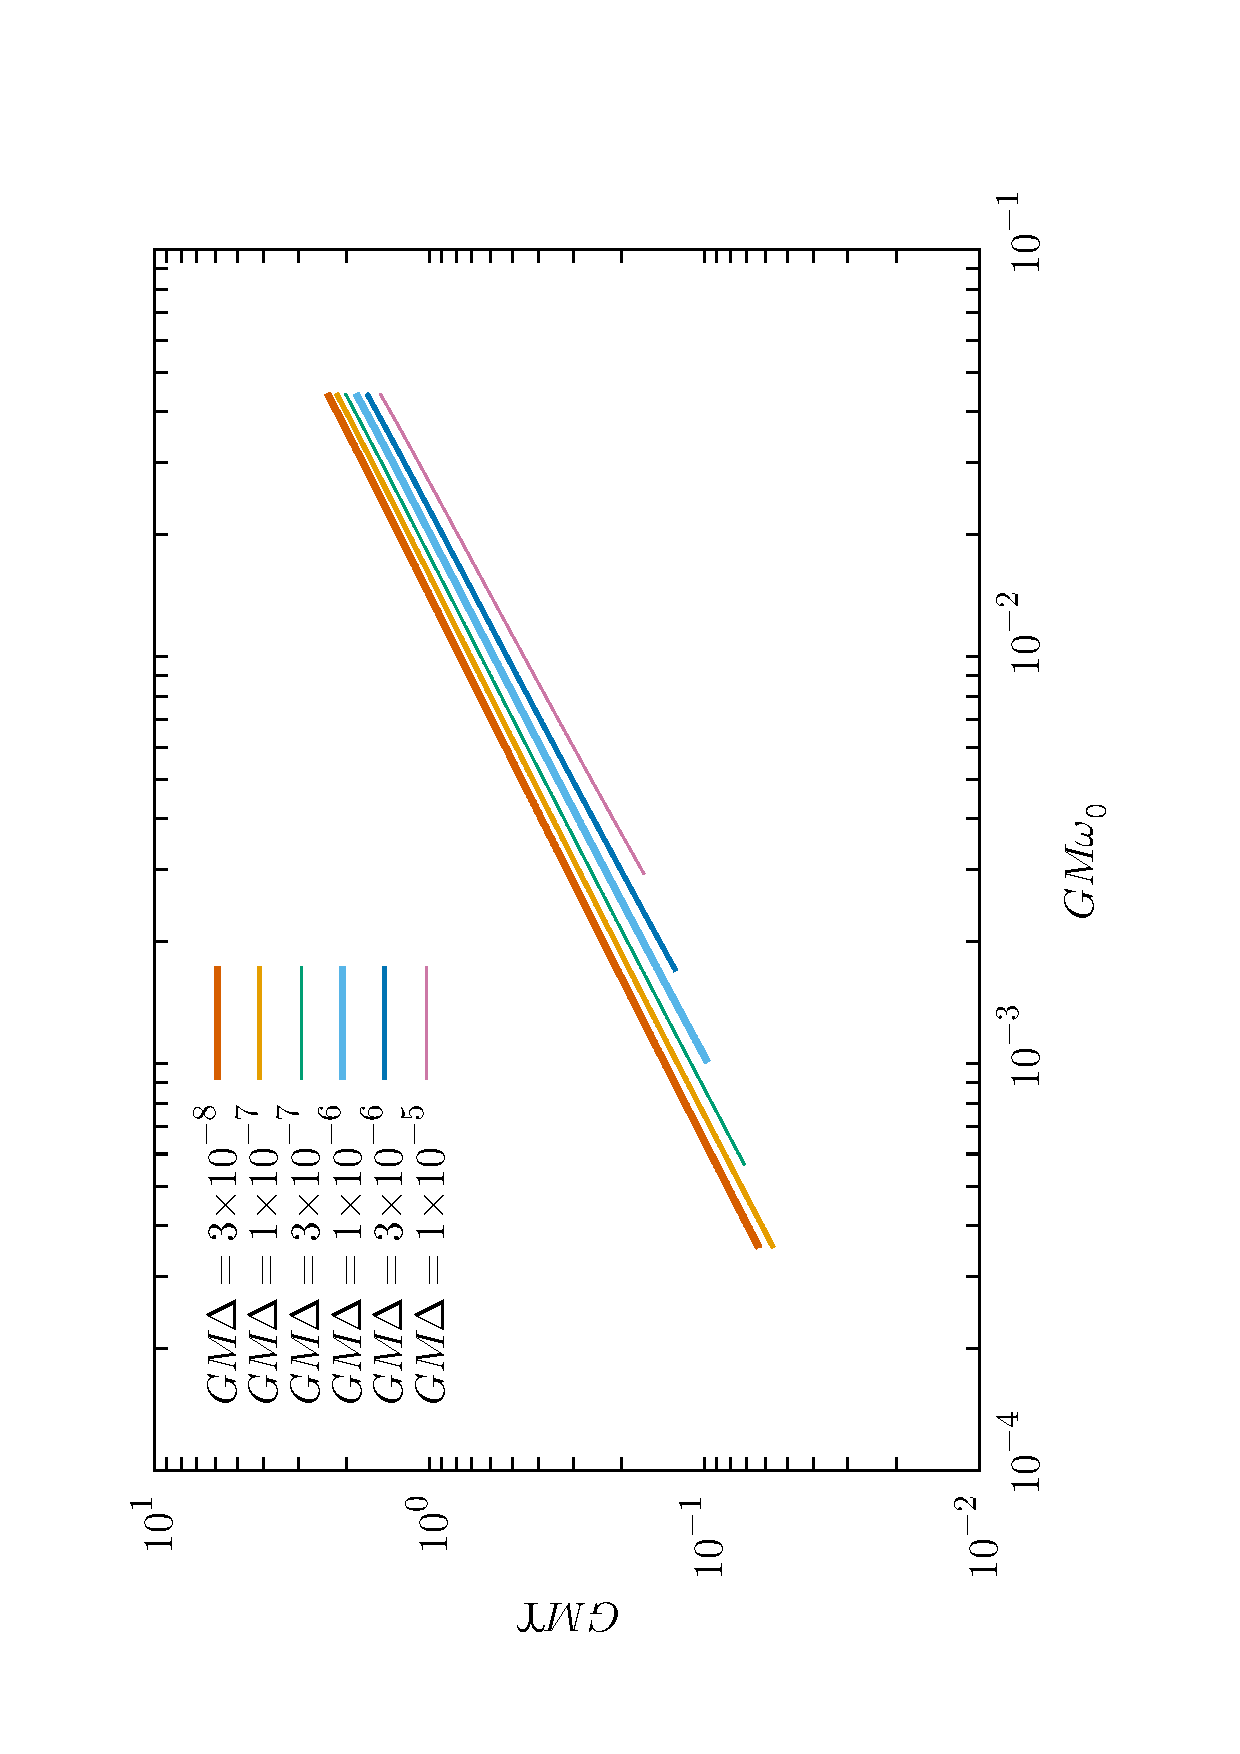
\includegraphics[angle=270, width=0.48\textwidth]{./images/EpicycleConstraintsa0}}
\quad\subfigure[For spin $a_\ast = 0.5$.]{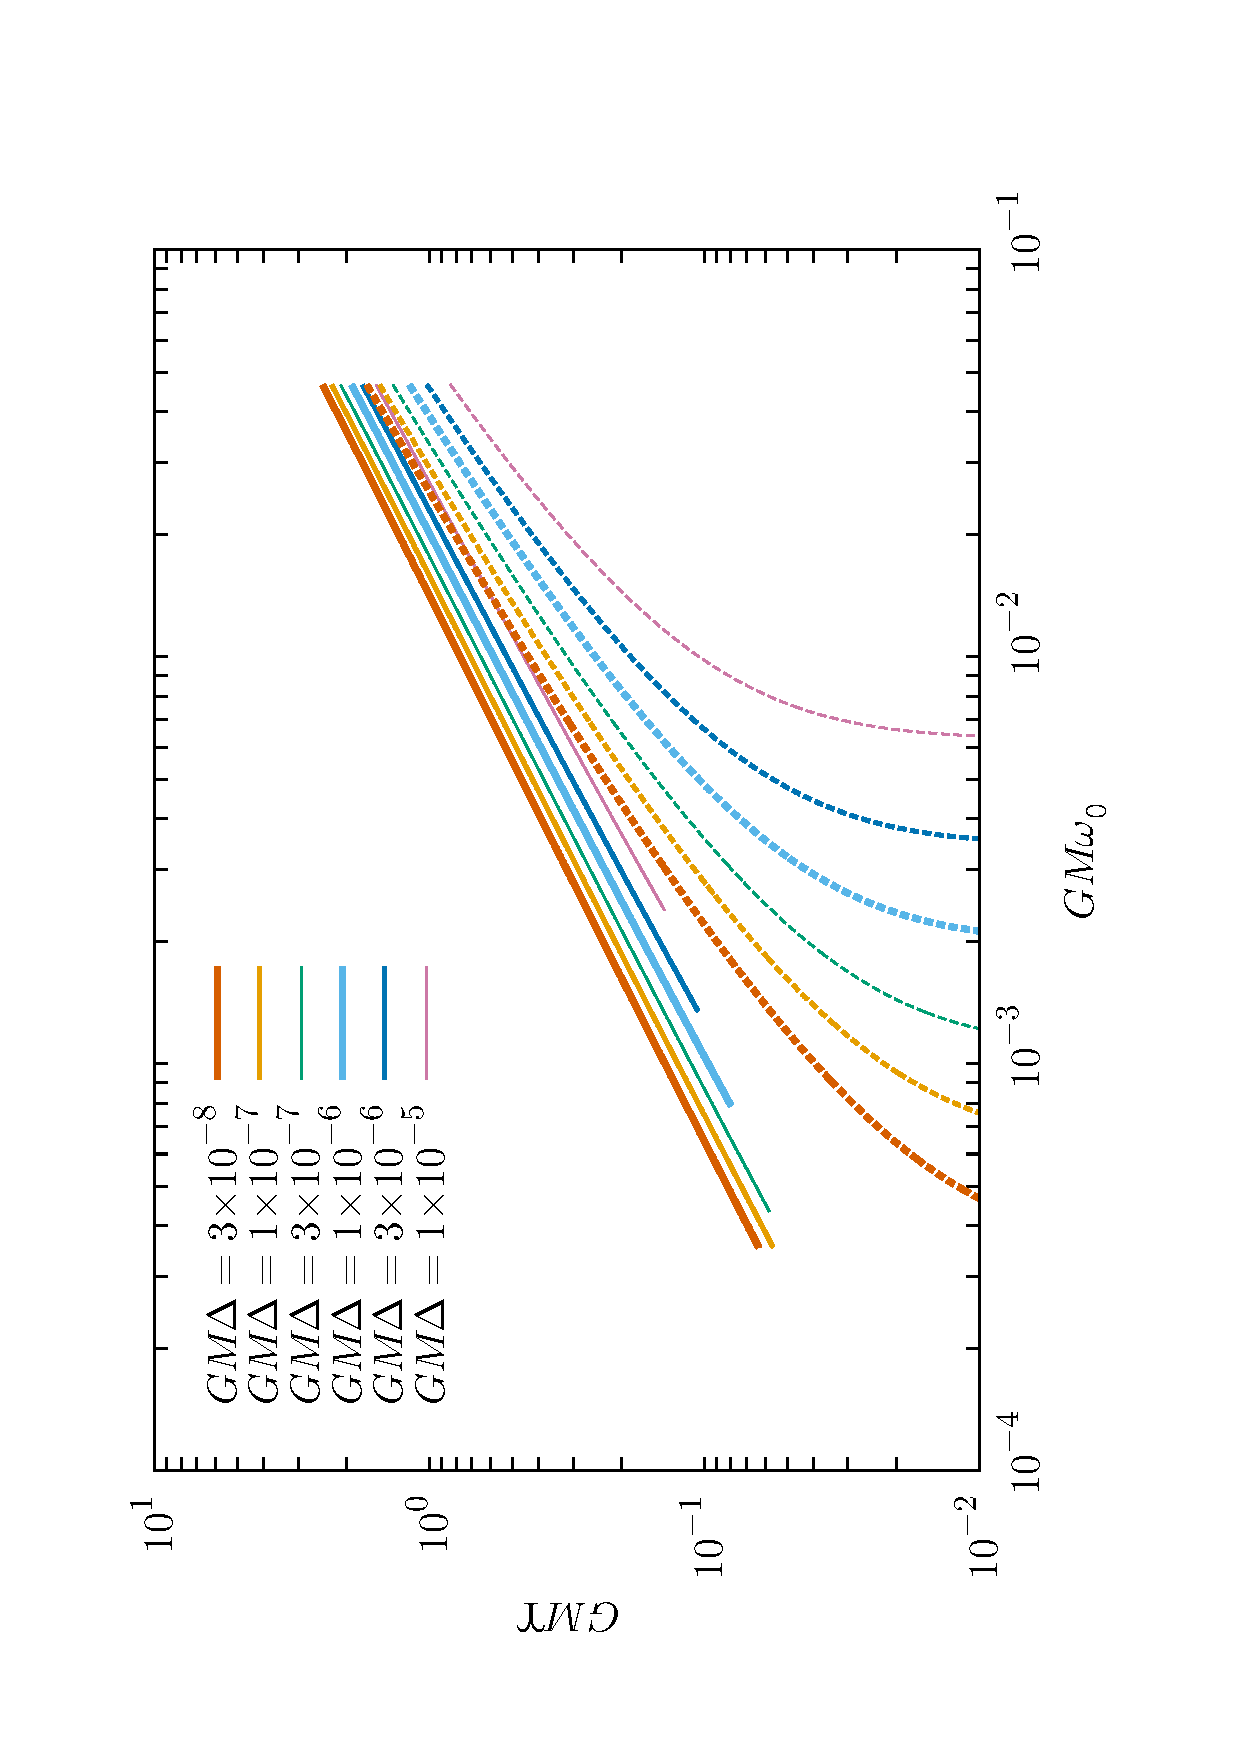
\includegraphics[angle=270, width=0.48\textwidth]{./images/EpicycleConstraintsa05}}
\caption{\label{fig:epifig}Region of parameter space in which $f(R)$ and Kerr trajectories can be distinguished. Curve corresponds to different values of the detectability criterion \eqnref{detcrit}, given in the key. Dashed lines are measurements of the vertical epicyclic frequency, solid lines are for measurements of the radial epicyclic frequency. The region below a curve could be distinguishable in a LISA observation with that detectability.}
\end{figure*}
Each curve represents a particular choice for $GM\Delta$: the region below the curve is detectable in an observation characterised by that choice. \Eqnref{detcrit} indicates that the curve $GM\Delta = 10^{-6}$ is what would be achieved in a one-year observation for a $10^6 M_\odot$ mass central object. The curves $GM\Delta = 10^{-5}/10^{-7}$ are the corresponding results for a $10^7/10^5M_\odot$ mass object, while the curve $GM\Delta = 3 \times 10^{-7}$ represents what would be achieved in a three-year observation. We show results for two choices of spin: $a_\ast = J/GM^2 = 0$ and $a_\ast = 0.5$. There is not much difference between the two. The vertical epicyclic frequency is only measurable for $a_\ast \neq 0$ as it coincides with the orbital frequency for $a_\ast = 0$ as a consequence of the spherical symmetry. Results are shown only for prograde orbits. For $a_\ast \neq 0$, we can compute results for retrograde orbits; these differ from the prograde results by an amount which is almost indistinguishable on the scale of the plots.

From \figref{epifig} we conclude that we could be able to distinguish spacetimes with $GM\Upsilon \lesssim 1 $. For a $10^6 M_\odot$ central object this corresponds to $\Upsilon \lesssim 10^{-9}\units{m^{-1}}$. Larger values are accessible at higher frequencies, but the inspiral would pass through that region quickly, and these orbits correspond to relatively small radii at which the weak-field approximations begin to break down, so we must be cautious extrapolating these results. Using this detectability criterion, the radial epicyclic frequency is always a more powerful probe than the vertical epicyclic frequency. This is expected; the latter is generally smaller in magnitude and so accumulates fewer cycles over a typical observation.

\section{Solar System and laboratory tests\label{sec:Tests}}

\subsection{Light bending \& the post-Newtonian parameter $\gamma$}

The parametrized post-Newtonian (PPN) formalism was created to quantify deviations from GR~(\citealt[chapter 4]{Will1993}; \citealt{Will2006}). It is ideal for Solar System tests. The only parameter we need to consider here is $\gamma$, which measures the space-curvature produced by unit rest mass. The PPN metric has components
\begin{equation}
g\super{PPN}_{00} = 1 - 2U; \qquad g\super{PPN}_{ij} = -(1 + 2\gamma U)\delta_{ij},
\end{equation}
where for a point mass
\begin{equation}
U(r) = \frac{GM}{r}.
\end{equation}
The metric must be in isotropic coordinates~(\citealt[section 40.1]{Misner1973}; \citealt[section 4.1(c)]{Will1993}). The $f(R)$ metric \eqnref{f(R)_Schw} is of a similar form, but there is not a direct correspondence because of the exponential.\footnote{Our $f(R)$ theory is equivalent to a Brans-Dicke theory with a potential and parameter $\omega\sub{BD} = 0$ \citep{Teyssandier1983, Wands1994}. We cannot use the familiar result $\gamma = (1 + \omega\sub{BD})/(2 + \omega\sub{BD})$ \citep{Will2006} as this was derived for Brans-Dicke theory without a potential \citep[section 5.3]{Will1993}.} It has been suggested that this may be incorporated by changing the definition of the potential $U$ \citep{Olmo2007c, Faulkner2007, Bisabr2010, DeFelice2010}, then
\begin{equation}
\gamma = \frac{3 - \exp(-\Upsilon r)}{3 + \exp(-\Upsilon r)}.
\end{equation}
As $\Upsilon \rightarrow \infty$, the GR value of $\gamma = 1$ is recovered. However, the experimental bounds for $\gamma$ are derived assuming that it is a constant \citep[section 6.1]{Will1993}. Since this is not the case, we shall rederive the post-Newtonian, or $\order{\varepsilon}$, corrections to photon trajectories for a more general metric. We define
\begin{equation}
\dd s^2 = \left[1+2\Psi(r)\right]\dd t^2 - \left[1 - 2\Phi(r)\right]\left(\dd x^2 + \dd y^2 + \dd z^2\right).
\end{equation}
To post-Newtonian order, this has nonzero connection coefficients
\begin{equation}
{\Gamma^0}_{0i} = \frac{\Psi'(r) x^i}{r}; \quad {\Gamma^i}_{00} = \frac{\Psi'(r) x^i}{r}; \quad
{\Gamma^i}_{jk} = \frac{\Phi'(r)\left(\delta_{jk}x^i - \delta_{ij}x^k - \delta_{ik}x^j\right)}{r}.
\end{equation}
The photon trajectory is described by the geodesic equation
\begin{equation}
\difftwo{x^\mu}{\sigma} + {\Gamma^\mu}_{\nu\rho}\diff{x^\nu}{\sigma}\diff{x^\rho}{\sigma} = 0,
\label{eq:Geodesic}
\end{equation}
for affine parameter $\sigma$. The time coordinate obeys
\begin{equation}
\difftwo{t}{\sigma} + {\Gamma^0}_{\nu\rho}\diff{x^\nu}{\sigma}\diff{x^\rho}{\sigma} = 0,
\end{equation}
so we can rewrite the spatial components of \eqnref{Geodesic} using $t$ as an affine parameter \citep[section 6.1]{Will1993}
\begin{equation}
\difftwo{x^i}{t} + \left({\Gamma^i}_{\nu\rho} - {\Gamma^0}_{\nu\rho}\diff{x^i}{t}\right)\diff{x^\nu}{t}\diff{x^\rho}{t} = 0.
\end{equation}
Since the geodesic is null we also have
\begin{equation}
g_{\mu\nu}\diff{x^\mu}{t}\diff{x^\nu}{t} = 0.
\end{equation}
To post-Newtonian accuracy these become
\begin{align}
\label{eq:Trajectory_1}
\difftwo{x^i}{t} = {} & -\left(\frac{\Psi'}{r} + \frac{\Phi'}{r}\left|\diff{\boldsymbol{x}}{t}\right|^2\right)x^i + 2\frac{\Psi' + \Phi'}{r}\boldsymbol{x}\cdot\diff{\boldsymbol{x}}{t}\diff{x^i}{t}, \\
0 = {} & 1 + 2\Phi - \left(1 - 2\Phi\right)\left|\diff{\boldsymbol{x}}{t}\right|^2.
\label{eq:Trajectory_2}
\end{align}
The Newtonian, or zeroth-order, solution of these is propagation in a straight line at constant speed \citep[section 6.1]{Will1993}
\begin{equation}
x^i\sub{N} = n^it; \qquad |\boldsymbol{n}| = 1.
\end{equation}
The post-Newtonian trajectory can be written as
\begin{equation}
x^i = n^it + x^i\sub{pN}
\end{equation}
where $x^i\sub{pN}$ is the deviation from the straight line. Substituting this into equations \eqref{eq:Trajectory_1} and \eqref{eq:Trajectory_2} gives
\begin{align}
\difftwo{\boldsymbol{x}\sub{pN}}{t} = {} & -\grad(\Psi + \Phi) + 2\boldsymbol{n}\cdot\grad(\Psi + \Phi)\boldsymbol{n}, \\
\boldsymbol{n}\cdot\diff{\boldsymbol{x}\sub{pN}}{t} = {} & \Psi + \Phi.
\end{align}
The post-Newtonian deviation only depends upon the combination $\Psi + \Phi$. From \eqnref{f(R)_Schw}
\begin{align}
\Psi(r) + \Phi(r) = {} & -\frac{2GM}{r} \nonumber \\*
 = {} & -2U(r).
\end{align}
This is identical to the form in GR. The result holds not just for a point mass, using \eqnref{h_metric},
\begin{align}
2\left(\Psi + \Phi\right) = {} & h_{00} + h_{ii} \qquad \text{(no summation)}\nonumber \\*
 = {} & \overline{h}_{00} + \overline{h}_{ii},
\end{align}
and since $\overline{h}_{\mu\nu}$ obeys \eqnref{Box_hmunu} exactly as in GR, there is no difference \citep{Zhao2011}. We conclude that an appropriate definition for the post-Newtonian parameter for light-bending is
\begin{equation}
\gamma = -\frac{g_{00} + g_{ii}}{2U} - 1 \qquad \text{(no summation)}.
\end{equation}
Using this, our $f(R)$ solutions have $\gamma = 1$. This agrees with the result found by \citet{Clifton2008}.\footnote{\citet{Clifton2008} also gives PPN parameters $\beta = 1$, $\zeta_1 = 0$, $\zeta_3 = 0$ and $\zeta_4 = 0$, all identical to the values in GR.} Consequently, $f(R)$-gravity is indistinguishable from GR in this respect and is entirely consistent with the current observational value of $\gamma = 1 + (2.1 \pm 2.3) \times 10^{-5}$ \citep{Will2006, Bertotti2003}.

This result has important implications. To first order, the gravitational lensing of light in $f(R)$-gravity is identical to that in GR. Therefore, we still need dark matter to explain lensing observations of galaxies and galaxy clusters \citep{Lubini2011}. $f(R)$-gravity is not an alternative to dark matter.

There are non-linear signatures of $f(R)$-gravity that may be observable with lensing measurements; however, these are too small to be currently observable \citep{Vanderveld2011}. We must use other experiments to put constraints upon $f(R)$.

\subsection{Planetary precession}

The epicyclic frequencies derived in \secref{Epicycle} can be used for the classic test of planetary precession in the Solar System.\footnote{Since the Sun is an extended body, we do not have to worry about BH solutions being identical in GR and $f(R)$-gravity here.} Radial motion perturbs the orbit into an ellipse. The amplitude of our perturbation $\delta$ gives the eccentricity $e$ of the ellipse \citep{Kerner2001a}. Unless $\omega_0 = \Omega\sub{rad}$ the epicyclic motion is asynchronous with the orbital motion: there is periapse precession. In one revolution the ellipse precesses about the focus by
\begin{equation}
\varpi = 2\pi\left(\frac{\omega_0}{\Omega\sub{rad}} - 1\right)
\end{equation}
where $\omega_0$ is the frequency of the circular orbit given in \eqnref{omz}. The precession is cumulative, so a small deviation may be measurable over sufficient time. Taking the non-rotating limit, the epicyclic frequency is
\begin{equation}
\Omega\sub{rad}^2 = \omega_0^2 \left[1 - \frac{3r\sub{S}}{\overline{r}} - \zeta(\Upsilon,r\sub{S},\overline{r})\right],
\end{equation}
defining the function
\begin{align}
\zeta = {} & r\sub{S}\left(\recip{\overline{r}} + \Upsilon\right)\frac{\exp(-\Upsilon r)}{3} + \frac{\Upsilon^2\overline{r}^2\exp(-\Upsilon r)}{3 + (1 + \Upsilon \overline{r})\exp(-\Upsilon r)} \left[1 - \frac{r\sub{S}}{\overline{r}} + r\sub{S}\left(\recip{\overline{r}} + \Upsilon\right)\frac{\exp(-\Upsilon r)}{3}\right].
\end{align}
This characterises the deviation from the Schwarzschild case: the change in the precession per orbit relative to Schwarzschild is
\begin{align}
\Delta \varpi = {} & \varpi - \varpi\sub{S} \\
 = {} & \pi\zeta,
\end{align}
using the subscript $\text{S}$ to denote the Schwarzschild value. To obtain the last line we have expanded to lowest order, assuming that $\zeta$ is small.\footnote{There is one term in $\zeta$ that is not explicitly $\order{\varepsilon}$. Numerical evaluation shows that this is $< 0.6$ for the applicable range of parameters.} Since $\zeta \geq 0$, the precession rate is enhanced relative to GR.

\Tabref{Precess} shows the orbital properties of the planets. We use the deviation in perihelion precession rate from the GR prediction to constrain the value of $\zeta$, and hence $\Upsilon$ and $a_2$.
%\squeezetable
\begin{table}[bht]%\footnotesize
\centering
\begin{tabular}{l D{.}{.}{2.8} D{.}{.}{3.8} c D{.}{.}{1.8}}
\toprule
 & \multicolumn{1}{c}{Semimajor axis} & \multicolumn{1}{c}{Orbital period} & Precession rate & \multicolumn{1}{c}{Eccentricity} \\
Planet & \multicolumn{1}{c}{$r/10^{11}\units{m}$} & \multicolumn{1}{c}{$(2\pi/\omega_0)/\mathrm{yr}$} & $\Delta \varpi \pm \sigma_{\Delta \varpi}/\mathrm{mas\,yr^{-1}}$ & \multicolumn{1}{c}{$e$} \\
\midrule
Mercury & 0.57909175 & 0.24084445 & $\phantom{0}{-0.040} \pm \phantom{0}0.050\phantom{0}$ & 0.20563069 \\
Venus & 1.0820893 & 0.61518257 & $\phantom{-0}0.24\phantom{0} \pm \phantom{0}0.33\phantom{00}$ & 0.00677323 \\
Earth & 1.4959789 & 0.99997862 & $\phantom{-0}0.06\phantom{0} \pm \phantom{0}0.07\phantom{00}$ & 0.01671022 \\
Mars & 2.2793664 & 1.88071105 & $\phantom{0}{-0.07}\phantom{0} \pm \phantom{0}0.07\phantom{00}$ & 0.09341233 \\
Jupiter & 7.7841202 & 11.85652502 & $\phantom{-0}0.67\phantom{0} \pm \phantom{0}0.93\phantom{00}$ & 0.04839266 \\
Saturn & 14.267254 & 29.42351935 & $\phantom{0}{-0.10}\phantom{0} \pm \phantom{0}0.15\phantom{00}$ & 0.05415060 \\
Uranus & 28.709722 & 83.74740682 & ${-38.9}\phantom{00} \pm 39.0\phantom{000}$ & 0.04716771 \\
Neptune & 44.982529 & 163.7232045 & ${-44.4}\phantom{00} \pm 54.0\phantom{000}$ & 0.00858587 \\
Pluto & 59.063762 & 248.0208 & $\phantom{-}28.4\phantom{00} \pm 45.1\phantom{000}$ & 0.24880766 \\
\bottomrule
\end{tabular}
\caption{Orbital properties of the eight major planets and Pluto. We take the semimajor orbital axis to be the flat-space distance $r$, not the coordinate $\widetilde{r}$. The eccentricity is not used in calculations, but is given to assess the accuracy of neglecting terms $\order{e^2}$. Semimajor axis, orbital period and eccentricity are taken from \citet{Cox2000}, the precession rate is from \citet{Pitjeva2009a}\label{tab:Precess}}
\end{table}
All the precession rates are consistent with GR predictions ($\Delta \varpi = 0$) within their uncertainties. Assuming that these uncertainties constrain the possible deviation from GR we can use them as bounds for $f(R)$ corrections. \Tabref{Constraint} shows the constraints for $\Upsilon$ and $a_2$ obtained by equating the uncertainty in the precession rate $\sigma_{\Delta \varpi}$ with the $f(R)$ correction, and similarly using twice the uncertainty $2\sigma_{\Delta \varpi}$.
\begin{table}[bht]%\footnotesize
\centering
\begin{tabular}{l D{.}{.}{2.2} D{.}{.}{5.1} D{.}{.}{2.2} D{.}{.}{5.1}}
\toprule
 & \multicolumn{2}{c}{Using $\sigma_{\Delta \varpi}$} & \multicolumn{2}{c}{Using $2\sigma_{\Delta \varpi}$} \\
Planet & \multicolumn{1}{c}{$\Upsilon/10^{-11}\units{m^{-1}}$} & \multicolumn{1}{c}{$|a_2|/10^{18}\units{m^2}$} & \multicolumn{1}{c}{$\Upsilon/10^{-11}\units{m^{-1}}$} & \multicolumn{1}{c}{$|a_2|/10^{18}\units{m^2}$} \\
\midrule
Mercury & 52.6 & 1.2 & 51.3 & 1.3 \\
Venus & 25.3 & 5.2 & 24.6 & 5.5 \\
Earth & 19.1 & 9.1 & 18.6 & 9.6 \\
Mars & 12.2 & 22 & 11.9 & 24 \\
Jupiter & 2.96 & 380 & 2.87 & 410 \\
Saturn & 1.69 & 1200 & 1.63 & 1200 \\
Uranus & 0.58 & 9800 &  0.56 & 11000 \\
Neptune & 0.35 & 28000 & 0.33 & 31000 \\
Pluto & 0.26 & 49000 & 0.25 & 55000 \\
\bottomrule
\end{tabular}
\caption{Bounds calculated using uncertainties in planetary perihelion precession rates. $\Upsilon$ must be greater than or equal to the tabulated value, $|a_2|$ must be less than or equal to the tabulated value.\label{tab:Constraint}}
\end{table}
The tightest constraint is obtained from the orbit of Mercury. Adopting a value of $\Upsilon \geq 5.3 \times 10^{-10}\units{m^{-1}}$, the cut-off frequency for the Ricci mode is $\geq 0.16\units{s^{-1}}$. Therefore it could lie in the upper range of the LISA frequency band \citep{Bender1998,Danzmann2003} or in the ground-based detector frequency range \citep{Abramovici1992, Abbott2009, Accadia2010}. The constraints are not as tight as those from GW observations; however, as we shall see in \secref{Fifth}, it is possible to place stronger constraints on $\Upsilon$ using laboratory experiments.

\subsection{Fifth-force tests\label{sec:Fifth}}

From the metric \eqref{eq:f(R)_Schw}, a point mass has a Yukawa gravitational potential \citep{Stelle1978, Capozziello2009a, Naf2010}
\begin{equation}
V(r) = \frac{GM}{r}\left[1 + \frac{\exp(- \Upsilon r)}{3}\right].
\end{equation}
Potentials of this form are well studied in fifth-force tests \citep{Will2006, Adelberger2009, Adelberger2003} which consider a potential defined by a coupling constant $\alpha$ and a length-scale $\lambdabar$ such that
\begin{equation}
V(r) = \frac{GM}{r}\left[1 + \alpha\exp\left(-\frac{r}{\lambdabar}\right)\right].
\end{equation}
We are able to put strict constraints upon our length-scale $\lambdabar_R$, and hence $a_2$, because our coupling constant $\alpha_R = 1/3$ is relatively large. This can be larger for extended sources: comparison with \eqnref{Uniform} shows that for a uniform sphere $\alpha_R = \Xi(\Upsilon L) \geq 1/3$.

The best constraints at short distances come from the E\"{o}t-Wash experiments, which use torsion balances \citep{Kapner2007a, Hoyle2004}. These constrain $\lambdabar_R \lesssim 8\times 10^{-5}\units{m}$. Hence we determine $|a_2| \lesssim 2 \times 10^{-9}\units{m^2}$. Similar results have been obtained by \citet{Cembranos2009}, and by \citet{Naf2010}. This would mean that the cut-off frequency for a propagating scalar mode would be $\gtrsim 4 \times 10^{12}\units{s^{-1}}$ which is much higher than expected for astrophysical objects.

Fifth-force tests also permit $\lambdabar_R$ to be large. This degeneracy can be broken using other tests; from \secref{Epicycle} we know that the large range for $\lambdabar_R$ is excluded by planetary precession rates. This is supported by a result of \citet{Naf2010} obtained using the results of Gravity Probe B \citep{Everitt2009}.

While the laboratory bound on $\lambdabar_R$ may be strict compared to astronomical length-scales, it is still much greater than the expected characteristic gravitational scale, the Planck length $\ell\sub{P}$. We might expect for a natural quantum theory that $a_2 \sim \order{\ell\sub{P}^2}$, but $\ell\sub{P}^2 = 2.612 \times 10^{-70}\units{m^2}$, thus the bound is still about $60$ orders of magnitude greater than the natural value. The only other length-scale that we could introduce is defined by the cosmological constant $\Lambda$. Using the concordance values $\Lambda = 1.202 \times 10^{-52}\units{m^{-2}}$ \citep{Bennett2012, Hinshaw2012}, we see that $\Lambda^{-1} \gg |a_2|$. It is intriguing combining these two length-scales we find ${\ell\sub{P}}/{\Lambda^{1/2}} = 1.474 \times 10^{-9}\units{m^2}$, which is of the order of the current bound. This is coincidence, since there is nothing fundamental about the current level of precision, but it would be interesting to see if the measurements could be improved to rule out a Yukawa interaction around this length-scale.

\section{Summary of $f(R)$-gravity\label{sec:f_Discuss}}

Over the course of two chapters, we have examined the possibility of testing $f(R)$-type modifications to gravity using future GW observations and other measurements. We have seen that gravitational radiation is modified in $f(R)$-gravity as the Ricci scalar is no longer constrained to be zero; in linearised theory there is an additional mode of oscillation, that of the Ricci scalar. This is can only propagate above a cut-off frequency, but once excited, does carry additional energy-momentum away from the source. The two transverse GW modes are modified from their GR counterparts to include a contribution from the Ricci scalar, which would allow us to probe the curvature of the strong-field source regions. However, further study is needed in order to understand how GWs behave in a region with background curvature, in particular, when $R$ is nonzero.

From linearised theory we have deduced the weak-field metrics for some simple mass distributions and found they are not the same as in GR. Birkhoff's theorem no longer applies in $f(R)$-gravity, and extended bodies have a different gravitational field than in GR. However, the BH metrics of GR remain solutions in $f(R)$-gravity. This restricts the potential GW observations that could be made to test $f(R)$ theories.

LISA observations of EMRIs are sensitive to small differences in the precession frequencies of orbits: even tiny differences accumulate into a measurable dephasing over the $\sim 10^5$ cycles LISA would observe. However, as BHs are identical in both GR and $f(R)$-gravity there would be no difference in the orbital frequencies. There would be a difference if the compact object was an exotic extended object; in this case deviations would only be detectable when $|a_2| \gtrsim 10^{17}\units{m^2}$, assuming an extreme-mass-ratio binary with a massive object of mass $\sim 10^6 M_\odot$. This is calculated using the weak-field, slow-rotation metric. There could still be differences in the evolution of the inspiral because of a difference in the self-force.

We calculated constraints that can be placed using Solar System observations of planetary precessions and laboratory experiments. While the LISA constraints could beat those from Solar System observations (which presently give $|a_2| \lesssim 1.2 \times 10^{18}\units{m^2}$), considerably stronger constraints have already been placed from fifth-force tests. Using existing results from the E\"ot-Wash experiment, we constrain $|a_2| \lesssim 2 \times 10^{-9}\units{m^2}$. For this range of $a_2$, we do expect the propagating Ricci mode to be excited by astrophysical systems as the cut-off frequency is too high. However, even in the absence of excitation of the Ricci mode, gravitational radiation in $f(R)$-gravity is still modified through the dependence of the transverse polarizations on the Ricci scalar. 

Although the constraints from astrophysical observations are much weaker than this laboratory bound, they are still of interest since they probe gravity at a different scale and in a different environment. It is possible that $f(R)$-gravity is not universal, but changes in different regions of space or at different energy scales. The $f(R)$ model could be regarded as an approximate effective theory, and the range of validity of a particular parameterization is limited to a specific scale. For example, the effective theory in the vicinity of a massive BH, where the curvature is large, could be distinct from the appropriate effective theory in the Solar System, where curvature is small; or $f(R)$ could evolve with cosmological epoch such that it varies with redshift. If the laboratory bound is indeed universal there should be no deviation in GW observations: detection of a deviation would prove both that GR is incomplete and that the effective $a_2$ varies with environment.

One method of obtaining variation in the behaviour of gravity is via the chameleon mechanism. Then $f(R)$-gravity is modified in the presence of matter \citep{Khoury2004, Khoury2004a, Brax2004}. In metric $f(R)$-gravity this is a non-linear effect arising from a large departure of the Ricci scalar from its background value \citep{DeFelice2010}. The mass of the effective scalar degree of freedom then depends upon the density of its environment \citep{Faulkner2007, Li2007}. In a region of high matter density, such as the Earth, the deviations from standard gravity would be exponentially suppressed due to a large effective $\Upsilon$; while on cosmological scales, where the density is low, the scalar would have a small $\Upsilon$, perhaps of the order $H_0/c$ \citep{Khoury2004, Khoury2004a}. The chameleon mechanism allows $f(R)$-gravity to pass laboratory, or Solar System, tests while remaining of interest for cosmology.\footnote{The need to reconcile laboratory experiments with a non-trivial $f(R)$ could be regarded as motivation for introducing the chameleon mechanism.} In the context of gravitational radiation, this would mean that the Ricci scalar mode could freely propagate on cosmological scales \citep{Corda2009}. Unfortunately, because the chameleon mechanism suppresses the effects of $f(R)$ in the presence of matter, this mode would have to be excited by something other than the acceleration of matter. Additionally, since electromagnetic radiation has a traceless energy-momentum tensor it cannot excite the Ricci mode.\footnote{The standard transverse polarizations of gravitational radiation have an energy-momentum tensor that averages to be traceless, although this may not be the case locally \citep{Butcher2010}; the contribution to the gravitational averaged energy-momentum tensor from a propagating Ricci mode does have a nonzero trace, see \eqnref{Pseudotensor}. In any case it is doubtful that gravitational energy-momentum could act as a source for detectable radiation.} To be able to detect the Ricci mode we must observe it well away from any matter, which would cause it to become evanescent: a space-borne detector such as LISA could be our only hope.

As the chameleon mechanism is inherently non-linear, it is difficult to discuss in terms of our linearised framework. Treating $f(R)$ as an effective theory, we could incorporate the effects of matter by taking the coefficients $\{a_n\}$ to be functions of the matter stress-energy tensor (or its trace). In this case, the results presented here would hold in the event that the coefficient $a_2$ is slowly varying, such that it may be treated as approximately constant in the region of interest. The linearised wave equations, \eqref{eq:Box_R} and \eqref{eq:Box_hmunu}, retain the same form in the case of a variable $a_2$, the only alteration would be that $a_2 R^{(1)}$ replaces $R^{(1)}$ as subject of the Klein-Gordon equation. In particular, the conclusion that $\gamma = 1$ is unaffected by the possibility of a variable $a_2$.

An interesting extension to the work presented here would be to consider the case when the constant term in the function $f(R)$, $a_0$, is nonzero. We would then be able to study perturbations with respect to (anti-)de Sitter space. This is relevant because the current $\Lambda$CDM paradigm indicates that we live in a universe with a positive cosmological constant \citep{Jarosik2011, Komatsu2011}. Such a study would naturally complement an investigation into the effects of background curvature on propagation \citep{Yang2011}.
